\documentclass[acmsmall, review]{acmart}

%%
%% \BibTeX command to typeset BibTeX logo in the docs
\AtBeginDocument{%
  \providecommand\BibTeX{{%
    Bib\TeX}}}

%% Rights management information.  This information is sent to you
%% when you complete the rights form.  These commands have SAMPLE
%% values in them; it is your responsibility as an author to replace
%% the commands and values with those provided to you when you
%% complete the rights form.
% \setcopyright{acmlicensed}
% \copyrightyear{2023}
% \acmYear{2023}
% \acmDOI{XXXXXXX.XXXXXXX}


%%
%% These commands are for a JOURNAL article.
\acmJournal{TALG}
% \acmVolume{37}
% \acmNumber{4}
% \acmArticle{111}
% \acmMonth{8}

%%
%% Submission ID.
%% Use this when submitting an article to a sponsored event. You'll
%% receive a unique submission ID from the organizers
%% of the event, and this ID should be used as the parameter to this command.
%%\acmSubmissionID{123-A56-BU3}

%%
%% For managing citations, it is recommended to use bibliography
%% files in BibTeX format.
%%
%% You can then either use BibTeX with the ACM-Reference-Format style,
%% or BibLaTeX with the acmnumeric or acmauthoryear sytles, that include
%% support for advanced citation of software artefact from the
%% biblatex-software package, also separately available on CTAN.
%%
%% Look at the sample-*-biblatex.tex files for templates showcasing
%% the biblatex styles.
%%

%%
%% The majority of ACM publications use numbered citations and
%% references.  The command \citestyle{authoryear} switches to the
%% "author year" style.
%%
%% If you are preparing content for an event
%% sponsored by ACM SIGGRAPH, you must use the "author year" style of
%% citations and references.
%% Uncommenting
%% the next command will enable that style.
%%\citestyle{acmauthoryear}


%%
%% end of the preamble, start of the body of the document source.


% \usepackage{arxiv} # uncomment for preprint

\usepackage[utf8]{inputenc} % allow utf-8 input
\usepackage[T1]{fontenc}    % use 8-bit T1 fonts
% \usepackage{hyperref}       % hyperlinks
\usepackage{url}            % simple URL typesetting
\usepackage{booktabs}       % professional-quality tables
\usepackage{amsfonts}       % blackboard math symbols
\usepackage{nicefrac}       % compact symbols for 1/2, etc.
\usepackage{microtype}      % microtypography
\usepackage{lipsum}
\usepackage{graphicx}
\let\subcaption\relax
\usepackage{caption}
\usepackage{subcaption}
% \usepackage{subfigure}
\usepackage{amsmath}
% \usepackage{amssymb}
\usepackage{amsthm}
\usepackage{algorithm}
\usepackage{algorithmic}
\usepackage{hyperref}
\usepackage{xr}
% \usepackage{subfig}
\usepackage{xcolor}


\DeclareMathOperator*{\argmax}{arg\,max}
\DeclareMathOperator*{\argmin}{arg\,min}
\DeclareMathOperator{\score}{score}

% Note that the amsmath package sets \interdisplaylinepenalty to 10000
% thus preventing page breaks from occurring within multiline equations. Use:
\interdisplaylinepenalty=2500
% after loading amsmath to restore such page breaks as IEEEtran.cls normally
% does. amsmath.sty is already installed on most LaTeX systems. The latest
% version and documentation can be obtained at:
% http://www.ctan.org/pkg/amsmath

\usepackage{placeins}
% \usepackage{algpseudocode}

% \algnewcommand\algorithmicforeach{\textbf{foreach}}
% \algdef{S}[FOR]{ForEach}[1]{\algorithmicforeach\ #1\ \algorithmicdo}

\usepackage{hyperref}

% Attempt to make hyperref and algorithmic work together better:

\begin{document}
\title{CLAM-Accelerated K-Nearest Neighbors Entropy-Scaling Search of Large High-Dimensional Datasets via an Actualization of the Manifold Hypothesis}

\author{Morgan E. Prior}
\email{meprior424@gmail.com}
\orcid{0009-0003-1553-1672}
\affiliation{%
  \institution{Department of Mathematics and Applied Mathematical Sciences\\University of Rhode Island}
  \city{Kingston}
  \state{Rhode Island}
  \country{USA}
  \postcode{02881}
}

\author{Thomas J. Howard III}
\email{thoward27@uri.edu}
\orcid{0000-0001-6051-2508}
\affiliation{%
  \institution{Department of Computer Science and Statistics\\University of Rhode Island}
  \city{Kingston}
  \state{Rhode Island}
  \country{USA}
  \postcode{02881}
}

\author{Oliver McLaughlin}
\email{olwmcjp@gmail.com}
\orcid{0009-0009-0830-0124}
\affiliation{%
  \institution{Department of Computer Science and Statistics\\University of Rhode Island}
  \city{Kingston}
  \state{Rhode Island}
  \country{USA}
  \postcode{02881}
}



\author{Najib Ishaq}
\authornote{Co-corresponding authors.}
\email{najib\_ishaq@zoho.com}
\orcid{0009-0000-4091-4219}
\affiliation{%
  \institution{Department of Computer Science and Statistics\\University of Rhode Island}
  \city{Kingston}
  \state{Rhode Island}
  \country{USA}
  \postcode{02881}
}

\author{Noah M. Daniels}
\authornotemark[1]
\email{noah\_daniels@uri.edu}
\orcid{0000-0002-9538-825X}
\affiliation{%
  \institution{Department of Computer Science and Statistics\\University of Rhode Island}
  \city{Kingston}
  \state{Rhode Island}
  \country{USA}
  \postcode{02881}
}



%%
%% By default, the full list of authors will be used in the page
%% headers. Often, this list is too long, and will overlap
%% other information printed in the page headers. This command allows
%% the author to define a more concise list
%% of authors' names for this purpose.
\renewcommand{\shortauthors}{Prior et al.}

\begin{abstract}
  % Many fields are experiencing a Big Data explosion, with data collection rates outpacing the rate of computing performance improvements predicted by Moore's Law. 
  % Researchers are often interested similarity search on such data. 
  % We present CAKES (CLAM-Accelerated $K$-NN Entropy Scaling Search), a novel algorithm for $k$-nearest-neighbor ($k$-NN) search which leverages geometric and topological properties inherent in large datasets.
  % CAKES assumes the manifold hypothesis and performs best when data occupy a low dimensional manifold, even if the data occupy a very high dimensional embedding space. 
  % We demonstrate performance improvements ranging from hundreds to tens of thousands of times faster when compared to state-of-the-art approaches such as FAISS and HNSW, when benchmarked on 5 standard datasets.
  % Unlike locality-sensitive hashing approaches, CAKES can work with any user-defined distance function.
  % When data occupy a metric space, CAKES exhibits perfect recall.

  We need to re-do this. 
\end{abstract}

\begin{CCSXML}
<ccs2012>
   <concept>
       <concept_id>10003752.10003809</concept_id>
       <concept_desc>Theory of computation~Design and analysis of algorithms</concept_desc>
       <concept_significance>500</concept_significance>
       </concept>
 </ccs2012>
\end{CCSXML}
\ccsdesc[500]{Theory of computation~Design and analysis of algorithms}
%%
%% Keywords. The author(s) should pick words that accurately describe
%% the work being presented. Separate the keywords with commas.
\keywords{Approximate Search, Manifold Hypothesis}


%%
%% This command processes the author and affiliation and title
%% information and builds the first part of the formatted document.
\maketitle

    \section{Introduction}
\label{sec:introduction}

Researchers are collecting data at an unprecedented scale.
In many fields, the sizes of datasets are growing exponentially, and this increase in the rate of data collection outpaces improvements in computing performance as predicted by Moore's Law~\cite{kahn2011future}.
This indicates that the performance computer hardware will not ``catch up'' to computational needs in the near future.
Often dubbed ``the Big Data explosion,'' this phenomenon has created a need for better algorithms to analyze large datasets.

Examples of large datasets include genomic databases, time-series data such as radio frequency signals, and neural network embeddings.
Large language models such as GPT~\cite{2020arXiv200514165B, OpenAI2023GPT4TR} and LLAMA-2~\cite{Touvron2023Llama2O}, and image embedding models~\cite{radford2021learning, dosovitskiy2020image} are a common source of neural network embeddings.
These embeddings are often high-dimensional, and the sizes of training and inference datasets for such networks are growing exponentially.
Among biological datasets, the GreenGenes project~\cite{desantis2006greengenes} provides a multiple-sequence alignment of over one million bacterial 16S sequences, each 7,682 characters in length, while SILVA 18S~\cite{10.1093/nar/gks1219} contains ribosomal DNA sequences of approximately 2.25 million genomes with an aligned length of 50,000 letters.
Among time-series datasets, the RadioML dataset~\cite{oshea2018radioml} contains approximately 2.55 million samples of synthetically generated signal captures of different modulation modes over a range of SNR levels.

Many researchers are especially interested in similarity search on these datasets. 
Similarity search enables a variety of applications, including recommendation~\cite{annoy} and classification systems~\cite{suyanto2022knnclassifier}. 
As the cardinalities and dimensionalities of datasets have grown, however, efficient and accurate similarity search has become extremely challenging; 
even state-of-the-art algorithms exhibit a steep tradeoff between recall and throughput~\cite{Malkov2016EfficientAR, johnson2019billion, annoy, aumuller2020ann}.

Given some measure of similarity between data points, e.g. a distance function, there are two common definitions of similarity search: $k$-nearest neighbor search ($k$-NN) and $\rho$-nearest neighbor search ($\rho$-NN).
$k$-NN search aims to find the $k$ most similar points to a query, while $\rho$-NN search aims to find all points within a similarity threshold $\rho$ of a query.

Previous works have used the term \textit{approximate} search to refer to $\rho$-NN search, but in this paper, we reserve the term \textit{approximate} for search algorithms which do not exhibit perfect recall when compared to a na\"{i}ve linear search.
In contrast, an \textit{exact} search algorithm exhibits perfect recall.

$k$-NN search is one of the most ubiquitous classification and recommendation methods in use~\cite{fix1952discriminatory, cover1967nearest}.
Na\"{i}ve implementations of $k$-NN search, whose time complexity is linear in the dataset's cardinality, prove prohibitively slow for large datasets or those whose cardinalities are growing exponentially.
While fast algorithms for $k$-NN search on large datasets exist, most do not exploit the geometric and topological structure inherent in these datasets.
Further, such algorithms are often approximate~\cite{gao2023high}, and while approximate search may be sufficient for some applications, the need for efficient and \textit{exact} search remains~\cite{ukey2023survey}.

For example, for a majority voting classifier, approximate $k$-NN search may agree with exact $k$-NN search for large values of $k$, but may be sensitive to local perturbations for smaller values of $k$.
This is especially true when classes are not well-separated~\cite{zhang2022imbalanced}.
Further, there is evidence that distance functions which do not obey the triangle inequality, such as cosine distance, perform poorly for $k$-NN search in biomedical settings~\cite{hu2016distance};
this suggests that approximate $k$-NN search could exhibit suboptimal classification accuracy in such contexts.

$\rho$-NN search also has a variety of applications.
For example, one could search for all genomes within a maximum edit distance of a query genome to find evolutionarily-related organisms~\cite{budowski2010fragbag}.
One could also search for all words within a maximum edit distance of a misspelled word to suggest corrections~\cite{ukkonen1985algorithms}.
Given an advertisement and a database of user profiles, one could search for all users whose profiles are ``similar enough'' to target the advertisement~\cite{zhang2020privacy}.
GPS and other location-based services use $\rho$-NN search to find nearby points of interest~\cite{zhang2020privacy} to a user's location.
In all of these cases, approximate $\rho$-NN search may be sufficient, but exact $\rho$-NN search is preferable.

This paper introduces CAKES (CLAM-Accelerated $K$-NN Entropy Scaling Search), a set of three novel algorithms for exact $k$-NN search.
We also present some improvements to the clustering and $\rho$-NN search algorithms in CHESS~\cite{ishaq2019clustered}, as well as improved genericity across distance functions.
We provide a comparison of CAKES's algorithms to several state-of-the-art algorithms for similarity search, FAISS~\cite{johnson2019billion}, HNSW~\cite{malkov2016hnsw}, and ANNOY~\cite{annoy}, on datasets from the ANN-benchmarks suite~\cite{aumuller2020ann}.
We also benchmark CAKES on a large genomic dataset, the SILVA 18S dataset~\cite{10.1093/nar/gks1219}, using Levenshtein~\cite{levenshtein1966binary} distance on unaligned genomic sequences, and a radio frequency dataset, the RadioML dataset~\cite{oshea2018radioml}, using Dynamic Time Warping (DTW)~\cite{gold2018dynamic} distance on complex-valued time-series.


\subsection{Related Works}
\label{sec:intoduction:related-works}

Recent search algorithms designed to scale with the exponential growth of data include Hierarchical Navigable Small World networks (HNSW)~\cite{Malkov2016EfficientAR}, InVerted File indexing (FAISS-IVF)~\cite{faissivf}, random projection and tree building (ANNOY)~\cite{annoy}, and entropy-scaling search~\cite{yu2015entropy, ishaq2019clustered}. However, some of these algorithms do not provide exact search (as defined in Section \ref{sec:introduction} above).


\subsubsection{HNSW}
\label{sec:introduction:related-works:hnsw}

Hierarchical Navigable Small World networks~\cite{Malkov2016EfficientAR} is an approximate $k$-NN search method based on navigable small world (NSW) networks~\cite{kleinberg2000navigation, boguna2009navigability} and skip lists. 
Similar to the NSW algorithm, HNSW builds a graph of the dataset, but unlike NSW, the graph is multi-layered.
The query point and each data point are inserted into the graph one at a time, and, upon insertion, the element is joined by an edge to the $M$ nearest nodes in the in the graph, where $M$ is a tunable parameter. 
The highest layer in which an element can be placed is determined randomly with an exponentially decaying probability distribution.
Search starts at the highest layer and descends to the lowest layer, greedily following a path of edges to the nearest node, until reaching the query point. 
To improve accuracy, the $efSearch$ hyperparameter can be changed to specify the number of closest nearest neighbors to the query vector to be found at each layer. 


\subsubsection{FAISS-IVF}
\label{sec:introduction:related-works:faiss-ivf}

InVerted File indexing (IVF)~\cite{faissivf, sacks1987multikey, kent1990signature} is a method for approximate $k$-NN search. 
The data are clustered into high-dimensional Voronoi cells, and whichever cell the query point falls into is then searched exhaustively, similarly to an early precursor to our work~\cite{yu2015entropy}.
The number of cells used is governed by the $n_{list}$ parameter. 
Increasing this parameter decreases the number of points being exhaustively searched, so it improves speed at the cost of accuracy.
To mitigate accuracy issues caused by a query point falling near a cell boundary, the algorithm has a tunable parameter $n_{probe}$, which specifies the number of additional adjacent or nearby cells to search.


\subsubsection{ANNOY}
\label{sec:introduction:related-works:annoy}

This algorithm~\cite{annoy} is based on random projection and tree building for approximate $k$-NN search.
At each intermediate node of the tree, two points are randomly sampled from the space, and the hyperplane equidistant from them is chosen to divide the space into two subspaces.
This process is repeated multiple times to create a forest of trees, and the number of times the process is repeated is a tunable parameter.
At search time, one can increase the number of trees to be searched to improve recall at the cost of speed.

\subsubsection{Entropy-Scaling Search}
\label{sec:introduction:related-works:entropy-scaling-search}

This search paradigm exploits the geometric and topological structure inherent in large datasets.
Importantly, as suggested by their name, entropy-scaling search algorithms have asymptotic complexity that scales with topological properties (such as the \textit{metric entropy} and \textit{local fractal dimension}, as defined in Section~\ref{sec:methods}) of the dataset, instead of its cardinality.
In 2019, we introduced CHESS (Clustered Hierarchical Entropy-Scaling Search)~\cite{ishaq2019clustered}, which extended entropy-scaling $\rho$-NN search from a flat clustering approach to a tree-based hierarchical clustering approach.
CLAM (Clustering, Learning and Approximation with Manifolds), originally developed to allow ``manifold mapping'' for anomaly detection~\cite{ishaq2021clustered}, is a refinement of the clustering algorithm from CHESS.
In this paper, we introduce CAKES, a set of three entropy-scaling algorithms for $k$-NN search, implemented in the Rust programming language. 
Using the cluster tree constructed by CLAM, CAKES extends CHESS to perform $k$-NN search. We also discuss improvements to the performance of CHESS's $\rho$-NN search.

    \section{Methods}
\label{sec:methods}

In this manuscript, we are primarily concerned with $k$-nearest neighbors search in a finite-dimensional space.
Given a dataset $\textbf{X} = \{x_1 \dots x_n\}$, we define a \emph{point} or \emph{datum} $x_i \in \textbf{X}$ as a singular observation (e.g., the genome of 
an organism, the neural embedding of a single image, or any entity on which we can define a \emph{distance function}).

We define a \emph{distance function} $f : \textbf{X} \times \textbf{X} \mapsto \mathbb{R}^+ \ \cup \ \{0\}$ as a function which, 
given two points $x, y \in \textbf{X}$, deterministically returns a non-negative real number.
We require that the distance function be symmetric (i.e., $f(x, y) = f(y, x)$ for all $x, y \in \textbf{X}$) and that the distance between two points $x$ and $y$ be zero if and only if $x = y$. 
In addition to these constraints, if the distance function obeys the triangle inequality, i.e., it is a \emph{distance metric}, then we guarantee that CAKES has perfect recall. 
Choice of distance function varies by type of data.
For example, with electromagnetic spectra, one could both Euclidean (L2) and Cosine distances.
With biological or string data, Hamming and Levenshtein distances are more appropriate.

Some of our algorithms for $\rho$- and $k$-nearest neighbors search rely on the \emph{local fractal dimension} at some point and length scale in the dataset.
We define local fractal dimension (LFD) as:

\begin{equation}
    \frac{\text{log}(\frac{|B_X(q, r_1)|}{|B_X(q, r_2)|})}{\text{log}(\frac{r_1}{r_2}) }
    \label{eq:methods:lfd}
\end{equation}

where $B_X(q, r)$ is the set of points contained in a ball of radius $r$ centered at a point $q$ in the dataset $\textbf{X}$.
We stress that this concept differs from the \emph{embedding dimension} of a dataset.
To illustrate the difference, consider SDSS's APOGEE dataset, wherein each datum is a nonnegative real-valued vector of length 8,575.
Hence, the \emph{embedding dimension} of this dataset is 8,575. 
However, due to physical constraints (namely, the laws of physics that govern stellar fusion and spectral emission lines), the data are constrained to a lower-dimensional manifold within the 8,575-dimensional embedding space.
The \emph{local fractal dimension} is an approximation of the dimensionality of that lower-dimensional manifold in the ``vicinity'' of a given point.
This notion that high-dimensional data collected from constrained generating phenomena typically only occupy a low-dimensional manifold within their embedding space is known as the \emph{manifold hypothesis}~\cite{fefferman2016testing}.

Figures 2 and 3 in~\cite{ishaq2019clustered} illustrate the low fractal dimensions of two datasets used with $\rho$-NN search in CHESS. 
We observe that for both APOGEE (Figure 2 in~\cite{ishaq2019clustered}) and GreenGenes (Figure 3 in~\cite{ishaq2019clustered}), other than the most extreme 10\% of clusters, virtually all clusters have a local fractal dimension of less than 2. 
This suggests that APOGEE and GreenGenes are good datasets for use with entropy-scaling search algorithms like CHESS and CAKES.


\subsection{Clustering}
\label{subsec:methods:clustering}

We define a \emph{cluster} as a set of points with a \emph{center}, a \emph{radius}, and an approximation of the \emph{local fractal dimension}.
The \emph{center} is the geometric median of a sample of points in the \emph{cluster}, and so it is a real data point.
The \emph{radius} is the maximum distance from any point in the cluster to the \emph{center}.
We estimate \emph{local fractal dimension} at the scale of the cluster radius and half the cluster radius.
Each cluster (unless it is a leaf cluster) has two child clusters in much the same way that a node in a binary tree has two child nodes.
We define the \emph{metric entropy} $\mathcal{N}_{\hat{r_c}}(X)$ of a data set $X$ under a hierarchical clustering scheme as a refinement of~\cite{yu2015entropy}, where metric entropy for a given cluster radius $r_c$ was the number of clusters of radius $r_c$ needed to cover all data.
Here, we use a hierarchical, divisive clustering approach, but with early stopping criteria; clusters which satisfy a user-specified stopping criterion (e.g. a specified cardinality or radius) are not further split.
Since we frame the asymptotic complexity of $\rho$-NN search in terms of the number of leaf clusters, the \emph{metric entropy} is best thought of in terms of the number of leaf clusters.

We start by building a divisive hierarchical clustering of the dataset with CLAM, using a similar recursive procedure as outlined in CHESS, but with the following improvements:
better selection of poles for partitioning and depth-first dataset reordering (see Section ~\ref{subsubsec:methods:clustering:dataset-depth-first-reordering}). 

CAKES assumes the manifold hypothesis. 
In other words, we assume that the dataset is embedded in a $D$-dimensional space, but that the data only occupy a $d$-dimensional manifold, where $d \ll D$. 
While we sometimes use Euclidean notions, such as voids and volumes, to talk about geometric and topological properties of clusters and of the manifold, CLAM does not rely on such notions; 
they serve merely as a convenient, intuitive way to talk about the underlying mathematics.


\subsubsection {Cluster Partitioning}
\label{subsubsec:methods:cluster-partitioning}

For a cluster $C$ with $|C|$ points, we begin by taking a random sample of $\sqrt{|C|}$ of its points, and computing pairwise distances between all points in the sample.
Based on those pairwise distances, we compute the \emph{geometric median} of this sample; 
i.e., the point which minimizes the sum of distances to all other points in the sample.
This geometric median is $C$'s \emph{center}.
The \emph{radius} of $C$ is the maximum distance from any point in $C$ to its center.
The point $l$ which is responsible for that radius (i.e., the furthest point from the center) is designated the \emph{left pole}.
The point $r$ which is furthest from $l$ is designated the \emph{right pole}.
We then partition the cluster into a \emph{left child} and \emph{right child}, where the left child contains all points in the cluster which are closer to $l$ than to $r$, and the right child contains all points in the cluster which are closer to $r$ than to $l$.
Without loss of generality, we assign to the left child those points which are equidistant from $l$ and $r$.
Starting from a root-cluster containing the entire dataset, we repeat this procedure until each leaf contains only one datum or some other user-specified stopping criterion is met.
This process is described in Algorithm \ref{alg:methods:clustering:partition}.


\begin{algorithm} % enter the algorithm environment
\caption{Partition(\emph{C})} % give the algorithm a caption
\label{alg:methods:clustering:partition} % and a label for \ref{} commands later in the document
\begin{algorithmic} % enter the algorithmic environment
    \STATE $m \Leftarrow \lfloor \sqrt{|C|} \rfloor$
    \STATE $seeds \Leftarrow m$ random points from $C.points$
    \STATE $c \Leftarrow$ geometric median of $seeds$
    \STATE $l \Leftarrow \argmax d(c,x) \ \forall \ x \in C.points$
    \STATE $r \Leftarrow \argmax d(l,x) \ \forall \ x \in C.points$
    \STATE $left \Leftarrow \{x | x \in C.points \land d(l,x) \le d(r,x)\}$
    \STATE $right \Leftarrow \{x | x \in C.points \land d(r,x) < d(l,x)\}$
    \IF{$|left| > 1$}
        \STATE Partition($left$)
    \ENDIF
    \IF{$|right| > 1$}
        \STATE Partition($right$)
    \ENDIF
\end{algorithmic}
\end{algorithm}


\subsubsection {Depth-First Reordering}
\label{subsubsec:methods:clustering:dataset-depth-first-reordering}

CAKES also improves upon CHESS by reordering the dataset in depth-first order of traversal of the tree.
In CHESS, each cluster stored a list of indices into the dataset, which we used during search to retrieve a cluster's points. 
Though this approach allowed us to retrieve the points in constant time, its memory cost was prohibitively high;
since each cluster stores indices for each of its points and, for a dataset with cardinality $n$, we store a total of $n$ indices at each depth in the tree.
Assuming a balanced tree and thus $\mathcal{O}\log(n)$ depth, this approach had $\mathcal{O}(n\log(n))$ memory cost.

One may improve this memory cost to $\mathcal{O}(n)$ by only storing these indices at the leaf cluster level.
This approach, however, introduces an $\mathcal{O}(n\log(n))$ time cost whenever we need to find the indices for 
a non-leaf cluster, since it requires a traversal of the subtree rooted at that cluster.

In this work, we introduce a new approach, wherein after building the cluster tree, we reorder the dataset so that points are stored in a depth-first order.
Then, within each cluster, we need only store the cluster's cardinality and an \emph{offset} to access the cluster's points from the dataset.
The root cluster has an offset of zero and a cardinality equal to the number of points in the dataset.
A left child has the same offset as that of its parent, and the corresponding right child has an offset equal to the left child's offset plus the left child's cardinality.
With no additional memory cost nor time cost for retrieving points during search, depth-first reordering offers significant improvements over the approach used in CHESS.


% % WE WILL USE THIS FOR COMPRESSION, so removing it for now 

% \subsubsection {Scaling Behavior of Cluster Radii}
% \label{subsubsec:methods:clustering:guaranteed-decrease-in-cluster-radii}

% While it may be tempting to assume that cluster radii decrease with each application of Partition (refer to Algorithm \ref{alg:methods:clustering:partition}), unfortunately, this assumption is incorrect. 
% Fortunately, we \emph{can} make some guarantees about the scaling behavior of cluster radii;
% in particular, we prove in this section that cluster radii will stop increasing after at most $d$ partitions, where $d$ is the fractal dimensionality of the dataset. 

% We can describe a $d$-dimensional distribution of data by choosing some set of $d$ mutually orthogonal axes.
% Let $2R$ be the maximum pairwise distance among the points in the dataset. 
% We choose the axes such that the two points that are $2R$ apart lie \emph{along one of the axes}. 
% Thus, a $d$-dimensional hyper-sphere of radius $R$ would bound the dataset. 
% In the worst case, (i.e., with a uniform-density distribution that fills the $d$-sphere), our axes will be such that $2R$ is the maximum pairwise distance \emph{along every axis}. 
% Such a distribution would also produce a balanced cluster tree.

% In this case, Partition will select a maximally distant pair of points to use as poles;
% without loss of generality, say it chooses two points at the extrema one of the $d$ axes. 
% After one partition, the maximum pairwise distance along that axis will be halved, i.e. bounded above by $R$.
% The next recursive Partition will select another of the $d$ axes, and once again, the distance along that axis will be bounded above by $R$
% Thus, after at most $d$ partitions, the maximum pairwise distance along each axis will be bounded above by $R$. 
% The overall (i.e., not restricted to one axis) maximum pairwise distance 
% will be bounded above by $R\sqrt{2}$ by, for example, two instances that lie at the extrema of different axes. 
% See Figure~\ref{fig:methods:scaling-behavior} for an example.

% Thus, starting with a cluster $C$ of radius $R$, after at most $d$ Partitions, the descendants of $C$ will each have radius
% bounded above by $\frac{R}{\sqrt{2}}$. In other words, cluster radii are guaranteed to decrease by a multiplicative factor of $\frac{\sqrt{2}}{2}$ after at 
% most $d$ partitions. 

% Note that, in practice, we never see a balanced clustering.
% Partition produces unbalanced trees due to the varying density of the sampling in different regions of the manifold and the low dimensional ``shape'' of the manifold.
% Further, in practice, the cluster radii decrease by a factor much larger than $\frac{\sqrt{2}}{2}$ with almost every partition;
% the upper bound of $d$ partitions is seldom realized. 

% \begin{figure}[ht!]
%     \centering
%     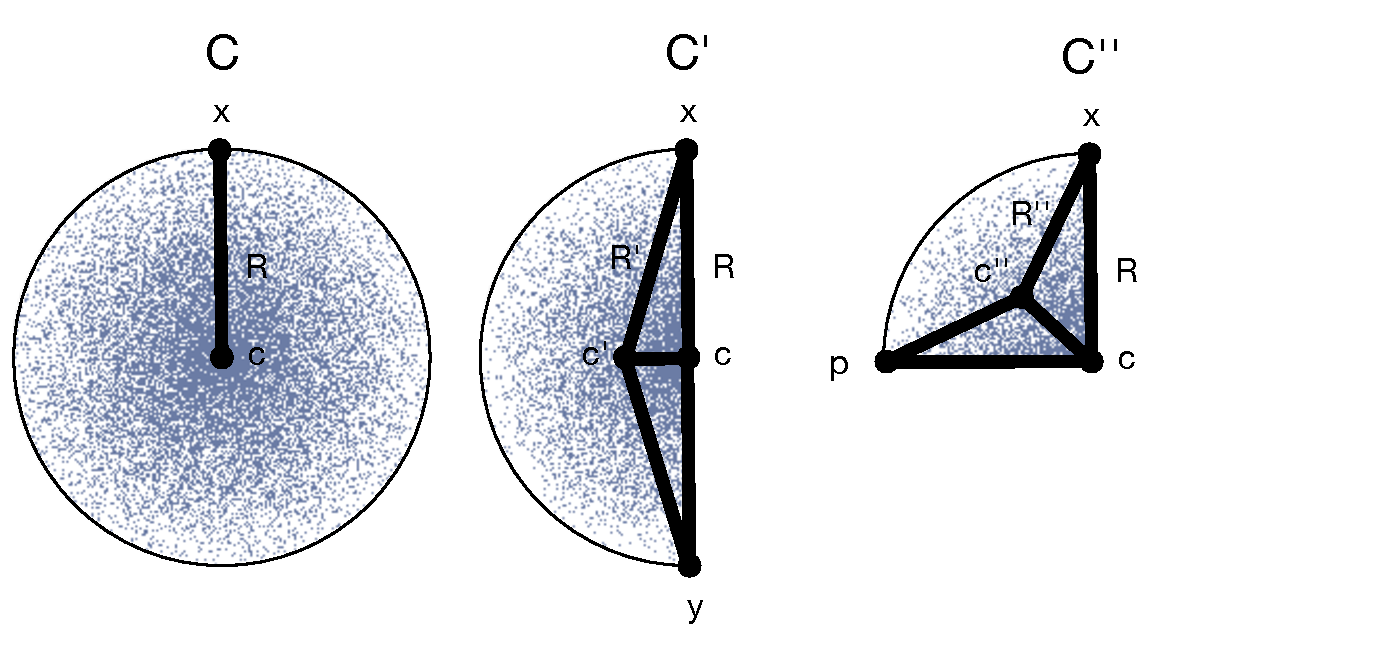
\includegraphics[width=3.4in]{images/geometry/geometry.pdf}
%     \caption{
%         Scaling behavior of radii on a uniform-density disk, which represents the worst-case scenario for a two-dimensional distribution. 
%         $R_0$ denotes the radius of the root cluster $C_0$, and $o_0$ denotes its center. 
%         After one application of Algorithm~\ref{alg:methods:clustering:partition}, we have $C_1$, with radius $R_1$ and center $o_1$.
%         The right triangle formed by $o_0$, $o_1$, and $y_+$ in $C_1$ shows that $R_0 < R_1$.
%         Hence, the radius of a child cluster can be larger than its parent.
%         However, after another application of Algorithm~\ref{alg:methods:clustering:partition}, we have consumed all $d$ orthogonal axes, 
%         as shown in $C_2$.
%         Now, clearly $R_2 < R_0$.
%         In fact, for each subsequent application of Algorithm~\ref{alg:methods:clustering:partition}, the radius of the resulting cluster is bounded above by $\frac{\sqrt{2}R}{2}$.
%     }
%     \label{fig:methods:scaling-behavior}
% \end{figure}


\subsubsection {Complexity}
\label{subsubsec:methods:clustering:clustering:complexity}

The asymptotic complexity of Partition is the same as described in~\cite{ishaq2019clustered}
By using an approximate partitioning with a $\sqrt{n}$ sample, we achieve $\mathcal{O}(n)$ cost of partitioning and $\mathcal{O}(n \log n)$ cost of building the tree.
This is a significant improvement over exact partitioning and tree-building, which have $\mathcal{O}(n^2)$ and $\mathcal{O}(n^2 \log n)$ costs respectively.


\subsection {Sharding and Auto-Tuning}
\label{subsec:methods:sharding-and-auto-tuning}

In this work, we also introduce a method of \emph{sharding} for datasets that cannot fit in memory.
This approach also leverages the fact that $\rho$-nearest neighbors search at the radius of the $k$-th farthest neighbor is typically much faster than $k$-nearest neighbors search.
In addition to sharding, we perform some na\"{i}ve auto-tuning to select the optimal $k$-NN algorithm to be used with a given dataset.

With this approach, we begin by taking a random sample of no more than 10\% of the data.
This sample is considered the first shard.
The exact proportion of the dataset in this random sample depends on the dimensionality of the dataset and a user-specified memory limit. 
We then split the rest of the dataset into more shards based on the user-defined memory limit.
For each shard, we build a cluster tree using Algorithm~\ref{alg:methods:clustering:partition}.
From the first shard, we consider all clusters at some user-specified depth in the tree, with a default depth of 10.
Using these clusters' centers as queries, and a user-specified value of $k$, we record the time taken for $k$-NN search on the sample using each of the four algorithms described in Section~\ref{subsec:methods:knn-search}.
We select the algorithm which had the lowest total search time over all the queries. 

Sharded search then proceeds as follows.
We use previously determined $k$-NN algorithm on the first shard. 
We use the distance to the $k$-th farthest neighbor to perform $\rho$-NN search on each subsequent shard. 
After searching each shard, we keep only the $k$-nearest neighbors so far, potentially decreasing the distance to the $k$-th farthest neighbor for search on the next shard.

Note that even though we select the optimal algorithm based on use with some user-specified value of $k$, we still allow search with any value of $k$.
Note also that the size of the shards is not necessarily consistent;
it is often optimal to have the first shard be smaller than the others, since the first shard is the only one for which we perform $k$-nearest neighbors search. 
However, making this first shard too small introduces the risk of significantly overestimating the radius (i.e., the distance to the $k$-th neighbor), resulting in much slower $\rho$-nearest neighbors search on the subsequent shards.
Finding the optimal ratio between the size of the first shard and the sizes of the remaining shards, as well as computing the expected level of error between the distance from the $k$-th closest neighbor in the first shard and the actual $k$-th closest neighbor, are topics for future work.
For datasets which \emph{do} fit in memory, we use the same approach to auto-tuning, but, since the entire dataset fits in memory, there is only one shard. 


\subsection{The Search Problem}
\label{subsec:methods:the-search-problem}
Having explained the clustering process, we can now pose the $k$-NN and $\rho$-NN search problems.
Given a query $q$, along with a distance function $f$ defined on a dataset $\textbf{X}$, $k$-nearest neighbors search aims to find 
the set $S_q$ such that  $|S_q| = k$ and $\forall x \in \textbf{X} \ \setminus \ S_q$, $f(x, q) > \max\{f(y, q): y \in S_q \}$;
that is, for a given $k$, find the $k$ closest points to $q$ in $ \textbf{X}$.
We also have the $\rho$-nearest neighbors search problem, which aims to find the set $\{x \in \textbf{X}: f(q, x) \leq \rho \}$;
that is, find all points in $\textbf{X}$ that are at most a distance $\rho$ from $q$.

Given a Cluster $C$, let $c$ be its center and $r$ be its radius. Our $\rho$- and $k$-NN algorithms make use of the following properties:

\begin{itemize}
    \item $\delta = f(q, c)$ is the distance from the query to the cluster center $c$.
    \item $\delta_{max} = \delta + r$ is the distance from the query to the theoretically farthest possible instance in $C$.
    \item $\delta_{min} = \text{max}(0, \delta - r)$ is the distance from the query to the theoretically closest possible instance in $C$.
\end{itemize}

We define a \emph{singleton} as a cluster which either contains a single point (i.e., has cardinality 1) or which contains 
duplicates of the same point (i.e., has cardinality greater than 1 but contains only one unique point).
A singleton clearly has zero radius, and so $\delta_{max} = \delta = \delta_{min}$ for these clusters.
Hence, we sometimes overload the above notation to also refer to distance from a query to a point;
in these cases, we also have that $\delta_{max} = \delta = \delta_{min}$.


\subsection{\texorpdfstring{$\rho$}{p}-Nearest Neighbors Search}
\label{subsec:methods:rnn-search}

We conduct $\rho$-nearest neighbors search as described in \cite{ishaq2019clustered}, but with the following improvement:
when a cluster overlaps with the query ball, instead of  always proceeding with both of its children, we proceed only with those children which also overlap with the query ball.
This improvement is described in Algorithm \ref{alg:methods:rnn-search}.

\begin{algorithm} 
    \caption{$\rho$-NN(\emph{cluster, query, r})} 
    \label{alg:methods:rnn-search} 
    \begin{algorithmic}
        \REQUIRE $r \geq 0$
        \REQUIRE $cluster \neq \emptyset$
        \STATE $results \Leftarrow \emptyset$
        \IF{$cluster.left \cap B_X(query, r) \neq \emptyset$}
            \IF{$cluster.left.\delta$ $\leq$ $r$ + $cluster.left.radius$}
                \STATE $\rho$-NN($cluster.left, query, r$)
            \ENDIF
        \ENDIF
        \IF{$cluster.right \cap B_X(query, r) \neq \emptyset$}
            \IF{$cluster.right.\delta$ $\leq$ $r$ + $cluster.right.radius$} 
                \STATE $\rho$-NN($cluster.right, query, r$)
            \ENDIF
        \ENDIF
        \IF{$cluster.isLeaf$}
            \FOR{$p \in cluster.points$}
                \IF{$p.\delta \leq r$}
                    \STATE $results.push((p, r))$
                \ENDIF
            \ENDFOR
        \ENDIF
        \STATE Return $results$
    \end{algorithmic}
\end{algorithm}

The asymptotic complexity of $\rho$-nearest neighbors is the same as in~\cite{ishaq2019clustered}, namely:

\begin{gather}
    \mathcal{O}\Bigg(
    \underbrace{\log_2 \mathcal{N}_{\hat{r_c}}(X)}_{\textrm{metric entropy}} +
    \overbrace{\left|B_X(q,r)\right|}^{\textrm{output size}}
    \underbrace{\left(1+\frac{2\hat{r_c}}{r}\right)^d}_{\textrm{scaling factor}}\Bigg)
    \label{hierarchical-complexity}
\end{gather}

where $\hat{r_c}$ is the \textit{mean} cluster radius of leaf clusters, $\mathcal{N}_{\hat{r_c}}(X)$ is the metric entropy at that radius, $B_X(q,r)$ is a ball of data points around the query $q$ at search radius $r$, and $d$ is the fractal dimension around the query in a region of radius $r$.


\subsection{\texorpdfstring{$k$}{k}-Nearest Neighbors Search}
\label{subsec:methods:knn-search}

In this section, we present four novel algorithms for exact $k$-nearest neighbors search: $k$-NN by Repeated $\rho$-NN, Sieve Search, Sieve Search with Separate Centers, and Greedy Sieve. 
We use a preliminary auto-tuning function to predict the variant (see Section~\ref{subsec:methods:sharding-and-auto-tuning}) which will perform 
best for a given dataset and value of $k$.
We then proceed with search using that variant on the first shard. 

In these algorithms, we typically use $H$, for \emph{hits}, to refer to the data structure which stores the closest points to the query found so far and
$Q$ to refer to the data structure which stores the clusters and points which are still in contention for being one of the nearest neighbors.


\subsubsection{\texorpdfstring{$k$}{k}-NN by Repeated \texorpdfstring{$\rho$}{p}-NN}
\label{subsubsec:methods:knn-search:repeated-rnn}

In this algorithm, we perform $\rho$-nearest neighbors search starting with a small search radius, and repeatedly increasing the radius until we find $k$ neighbors.

Let $H$ be the set of nearest neighbors found thus far.
Search starts with a radius $m$ equal to the radius of the root cluster divided by the cardinality of the dataset.
We perform $\rho$-NN search with radius $m$. 
If no points are within a distance $m$ of the query, we increase the radius by a factor of 2 and perform $\rho$-NN search again, repeating until at least one point is found.

Once $|H| > 0$, we continue to perform $\rho$-NN search, but instead of increasing the radius by a factor of 2 on each iteration, we increase it by a factor determined by the local fractal dimension in the region of the dataset around the query ball. 
In particular, we increase the radius by a factor of

\begin{equation}
    \min \left(2, \left({\frac{k}{|H|}}\right)^{\frac{1}{\mu}}\right)
    \label{eq:repeated-rnn-factor}
\end{equation}

where $\mu$ is the harmonic mean of the local fractal dimensions (abbreviated lfd in algorithm below) of each cluster which contains one of the nearest neighbors found thus far.
We use the harmonic mean to ensure that $\mu$ is not dominated by outlier clusters with very high fractal dimension. 
Intuitively, the factor by which we increase the radius should also be \emph{inversely} related to the number of points found so far. 
Additionally, when the local fractal dimension at the radius scale from the previous iteration is low, this suggests that the data are relatively concentrated in that region.
In other words, a small increase in the radius would likely encounter unoccupied space around the manifold, so a larger radial increase is needed.
Thus, the factor of radius increase should be \emph{inversely} related to the local fractal dimension.
Once $|H| >= k$, we sort the points by their distance to the query and return the $k$ closest points.

\begin{algorithm} % enter the algorithm environment
    \caption{Repeated $\rho$-NN(\emph{root, query, k})} % give the algorithm a caption
    \label{alg:knn-by-rnn} % and a label for \ref{} commands later in the document
    \begin{algorithmic} % enter the algorithmic environment
        \STATE $H \Leftarrow$ $\emptyset$
        \STATE $m \Leftarrow$ $\frac{root.radius}{|root|}$
        \WHILE {$H = \emptyset$}
            \STATE $H.push(\rho$-NN$(root, query, m)$)
            \STATE $m \Leftarrow 2m$
        \ENDWHILE
        \WHILE {$|H| < k$}
            \STATE $Q \Leftarrow \{ C: \exists p \in H \land p \in C \}$
            \STATE $\mu \Leftarrow \frac{|Q|}{\sum_{C \in Q} \frac{1}{C.lfd}} $
            \STATE $m \Leftarrow \min \left(2, \left({\frac{k}{|H|}}\right)^{\frac{1}{\mu}}\right)$
            \STATE $H.push(\rho$-NN$(root, query, m)$)
        \ENDWHILE
        \STATE $H.sort()$
        \STATE Return $H[0 \cdots k-1]$
    \end{algorithmic}
    \end{algorithm}


\subsubsection{Complexity of \texorpdfstring{$k$}{k}-NN by Repeated \texorpdfstring{$\rho$}{p}-NN Search}
\label{subsubsec:methods:repeated-rnn-complexity}

Our complexity bounds for $k$-NN by Repeated $\rho$-NN rely on the assumption that the query point is sampled from the same distribution (i.e. arises from the same generating phenomenon) as the rest of the data.
Given the uses of $k$-NN search in practice, this assumption is not unreasonable.
From this assumption, we can infer that the local fractal dimension at the query point does not differ significantly from the mean local fractal dimension of clusters nearby the query.

We find it useful to adopt the terminology used in \cite{ishaq2019clustered} and \cite{yu2015entropy}, and address \emph{coarse search} and \emph{fine search} separately.
Coarse search refers to the process of identifying clusters which have overlap with the query ball (i.e., which are likely to contain one of the $k$ nearest neighbors). 
Fine search refers to the process of identifying the $k$ nearest neighbors among the points in those clusters identified by coarse search.

In ~\cite{ishaq2019clustered}, we claimed that the complexity of coarse search for $\rho$-NN is $\mathcal{O}(\log\mathcal{N}_{\hat{r_c}}(X))$, 
where $\mathcal{N}_{\hat{r_c}}(X)$ is the metric entropy of the dataset $X$. 
To adjust this bound for $k$-NN by Repeated $\rho$-NN, we must estimate the number of iterations of $\rho$-NN needed to find at least $k$ neighbors.

Based on the assumption that the local fractal dimension at the query point is not significantly different than that of nearby clusters, the factor from Equation \ref{eq:repeated-rnn-factor} suggests that in the expected case, we need only two iterations of $\rho$-NN to find $k$ neighbors:
one iteration to find at least one neighbor, and the one more to find enough remaining neighbors.
Since this is a constant factor, it does not affect the asymptotic complexity of coarse search, and thus we have that the complexity of coarse search for $k$-NN by Repeated $\rho$-NN is $\mathcal{O}(\log_2\mathcal{N}_{\hat{r_c}}(X))$.

To determine the asymptotic complexity of fine search, we must estimate $|H|$, the expected number of hits we examine.
With $\rho$-NN search, $H$ is the union of clusters which are within a distance of $r + \hat{r_c}$ from the query, where $r$ is the search radius, and $\hat{r_c}$ is the mean radius of leaf clusters, as in \cite{yu2015entropy}.
With $k$-NN by Repeated $\rho$-NN, however, the value of $r$ is dependent on the distance to the $k$th nearest neighbor, which is query-dependent.
Thus, for $k$-NN by Repeated $\rho$-NN, we adjust the definition of $H$ to be the union of clusters which are within a distance of $r' + \hat{r_c}$ from the query, where $r'$ is the distance to the $k$th nearest neighbor and $\hat{r_c}$ is defined as before.

The work in~\cite{yu2015entropy} showed that

\begin{equation*}
    |H| \leq \gamma |B(q, r')|\left(1+ \frac{2\hat{r_c}}{r'}\right)^d
\end{equation*}

where $\gamma$ is a constant. 
By definition of 
$r'$, we have that $|B(q, r')| = k$. Thus, we have that

\begin{equation}
    |H| \leq \gamma k\left(1+ \frac{2\hat{r_c}}{r'}\right)^d
    \label{eq:methods:knn-by-rnn-fine-search}
\end{equation}

It remains to provide an estimate for $r'$. 
To do this, we once again rely on the assumption that the query is from the same distribution as the rest of the data, and thus the local fractal dimension at the query point is not significantly different than that of nearby clusters.

We let $\hat{d}$ be the mean of the local fractal dimensions of the clusters near the query point (i.e., the cluster identified during coarse search).
While ordinarily we compute local fractal dimension by comparing cardinalities of two balls with two different radii centered at \emph{the same} point, in order to estimate $r'$, we instead compare the cardinality of a ball \emph{around the query} of radius $r'$ to the mean cardinality $\hat{C}$ of clusters near the query at a radius equal to the mean of their radii $\hat{r}$.
We justify this approach by noting that, since the query is from the same distribution as the rest of the data, we could replace the query with the center of one of the clusters near it without significantly changing the local fractal dimension at the query point. 

By Equation ~\ref{eq:repeated-rnn-factor}, we then have that

\begin{equation*}
    \hat{d} = \frac{\log{}\frac{\hat{C}}{k}}{\log{}\frac{\hat{r}}{r'}}
\end{equation*}

Since $\hat{d}$, $\hat{C}$, $\hat{r}$, and $k$ are all known values, we can solve equation~\ref{eq:methods:knn-by-rnn-fine-search} for $r'$ to get

\begin{equation*}
    r' = \hat{r}\left(\frac{k}{\hat{C}}\right)^{\frac{1}{\hat{d}}}
\end{equation*}

Simplifying the expression for fine search, we have that

\begin{equation*}
    k\left(1+ \frac{2\hat{r_c}}{\hat{r}}\left(\frac{k}{\hat{C}}\right)^{\frac{-1}{\hat{d}}}\right)^d
\end{equation*}

Since we are dealing with asymptotic complexity, we can ignore the additive factor of $1$.
Putting our bounds for coarse and fine search together, we have that $k$-NN by Repeated $\rho$-NN has a complexity of



\begin{gather}
    \mathcal{O}\Bigg(
    \underbrace{\log_2{\mathcal{N}_{\hat{r_c}}(X)}}_{\textrm{metric entropy}} + 
    \overbrace{k}^{\textrm{output size}}
    \underbrace{\left(\frac{2\hat{r_c}}{\hat{r}}\right)^d\left(\frac{k}{\hat{C}}\right)^{\frac{-d}{\hat{d}}}}_{\textrm{scaling factor}}\Bigg)
    \label{eq:methods:knn-by-rnn-complexity}
\end{gather}

where $\mathcal{N}_{\hat{r_c}}(X)$ is the metric entropy of the dataset, $d$ is the dimensionality of the dataset, and $k$ is the number of nearest neighbors.
We note that the fraction $\frac{-d}{\hat{d}}$ should be relatively close to 1 unless fractal dimension is highly variable in a small region (that is, $\hat{d}$ differs significantly from $d$).


\subsubsection{Sieve}
\label{subsubsec:methods:knn-search:sieve}

In this algorithm, we begin by letting $Q$ be a list of clusters and points, starting with only the root cluster. 
While $Q$ contains at least one cluster (i.e., $Q$ is not a list of only points), we repeat the process described in 
the following paragraphs. 

First, we aim to find the element $q_{\tau} \in Q$ with the smallest $\delta_{max}$ such that 
$q_{\tau}$ and all elements in $Q$ with smaller $\delta_{max}$ collectively contain at least $k$ points. 

To find this element, we use a process similar to the Partition algorithm used in Quicksort~\cite{10.1093/comjnl/5.1.10}, adjusted to account for the varying cardinalities of clusters in $Q$ by having each cluster count a number of times equal to its cardinality.
Our modified version of this algorithm finds the smallest index $i$ such that all elements in $Q$ with $\delta_{max}$ less than or equal to $Q[i]$'s $\delta_{max}$ collectively have cardinality greater than or equal to $k$.
We consider $Q[i]$ to be our $q_{\tau}$, and our threshold $\tau$ to be $Q[i]$'s $\delta_{max}$.

We then remove from $Q$ any element whose $\delta_{min}$ is greater than $\tau$.
Then we remove all leaf clusters from $Q$ and add their points to $Q$ instead.
Finally, we replace all non-leaf clusters in $Q$ with their children. 

We continue this process until $Q$ contains only points.
At this point, we just use the Quicksort Partition algorithm once more to find the $k$th nearest neighbor and return all points to the left of it.

This process is described in Algorithm~\ref{alg:methods:sieve}. 

\begin{algorithm} % enter the algorithm environment
    \caption{Sieve(\emph{root, query, k})} % give the algorithm a caption
    \label{alg:methods:sieve} % and a label for \ref{} commands later in the document
    \begin{algorithmic} % enter the algorithmic environment
        \REQUIRE $root$, $query$, $k$
        \REQUIRE $root.cardinality \geq k$
        \STATE $Q \Leftarrow$ [$root$]
        \WHILE{$|Q| > k$}
            \STATE $i \Leftarrow QuicksortPartition(Q, k)$
            \STATE $\tau \Leftarrow Q[i].\delta_{max}$
            \FOR {$q \in Q$}
                \IF {$q.\delta_{min} > \tau$}
                    \STATE $Q.pop(q)$
                \ENDIF
            \ENDFOR
            \FOR {$q \in Q$}
                \IF {$q.isLeaf \lor |q| \leq k$}
                    \STATE $Q.append(q.points)$
                \ELSE
                    \STATE $[l, r] \Leftarrow q.children$
                    \STATE $Q.append([l, r])$   
                \ENDIF
                \STATE $Q.remove(q)$
            \ENDFOR 
        \ENDWHILE
        \STATE Return $Q$
    \end{algorithmic}
\end{algorithm}


\subsubsection{Sieve with Separate Centers}
\label{subsubsec:methods:knn-search:sieve2}

This algorithm is the same as Sieve, but with the following modification:
clusters in $Q$ are represented twice -- once as their center and once as the rest of their points.
The clusters' multiplicities in $Q$ are adjusted to be one less than their cardinalities.
Because we have that for any cluster $C$, $C.\delta \leq C.\delta_{max}$, representing the cluster center separately from the rest of the points causes the threshold $\tau$ to decrease more quickly, thus allowing us to eliminate some clusters from $Q$ earlier in the process. 


\subsubsection{Greedy Sieve}
\label{subsubsec:methods:knn-search:greedy-search}

We first let $Q$ be a min-queue of clusters prioritized by $\delta_{min}$.
$Q$ starts containing only the root cluster.
We also let $H$ be a fixed-size ($k$) max-queue of points prioritized by $\delta$.
$H$ starts empty.

While $H$ has fewer than $k$ points or $\delta$ of the top priority element in $H$ is greater than $\delta_{min}$ of the top priority element in $Q$, we do the following:

\begin{enumerate}
\item While the top priority element $q$ in $Q$ is not a leaf, pop it from $Q$ and push its children to $Q$.
\item For each point $p \in q$, push $p$ to $H$. 
\item Pop from $H$ until $H$ has $k$ points. 
\end{enumerate}

After this process, the points left in $H$ are the $k$ nearest neighbors of $q$.
This algorithm is described in Algorithm~\ref{alg:greedy-sieve}.

\begin{algorithm} 
\caption{Greedy Sieve(\emph{root, query, k})} 
\label{alg:greedy-sieve} 
\begin{algorithmic}
    \STATE $Q \Leftarrow$ priority queue
    \STATE $Q.push(root)$
    \STATE $H \Leftarrow$ priority queue
    \WHILE{$|H| < k \lor H.peek.\delta > Q.peek.\delta_{min}$}
        \WHILE{$\neg Q.peek.isLeaf$}
            \STATE $[l, r] \Leftarrow Q.pop().children$
            \STATE $Q.push([l, r])$
        \ENDWHILE
        \STATE $leaf \Leftarrow Q.pop()$
        \STATE $H.push(leaf)$
        \WHILE{$|H| > k$}
            \STATE $H.pop()$
        \ENDWHILE
    \ENDWHILE
    \STATE Return $H$
\end{algorithmic}
\end{algorithm}


\subsubsection{Complexity of Sieve Algorithms}
\label{paragraph:methods:sieve-complexity}

We group the Sieve-based algorithms together, as their complexity analyses are similar.
The complexity of Sieve and Sieve with Separate Centers is dominated by the expected cost of Quicksort's partition algorithm to calculate thresholds.
This method is linear in the size of the input list $Q$, so we must estimate the size of $Q$ on each iteration. 

We start by considering clusters whose cardinalities are within a small factor of $k$, say a factor of 2.
The distribution of such clusters will mimic the distribution of points in the dataset. 
From this assumption, we can infer that number of clusters which overlap with the query ball is a function of the local fractal dimension near the query.
In particular, we assume that the number of clusters which overlap the query ball is bounded above by 2$d$, where $d$ is the local fractal dimension of the dataset near the query point, e.g. we could have a cluster overlapping the query ball at each end of each of the $d$ axes.

In the worst case scenario, where the data are distributed with uniform density in their embedding space, it takes at most $\log{\frac{n}{2k}}$ iterations of Sieve to partition clusters enough that their cardinalities are at most $2k$.
However, since high cardinality clusters occur only at low depths in the tree, the length of $Q$ for those iterations is relatively low. 

After the first $\log{\frac{n}{2k}}$ iterations, we have that the cardinalities of clusters in $Q$ are at most $2k$, at which point, based on our assumption, we have that the length of $Q$ is close to $2d$.
Therefore, the asymptotic complexity of the sieve algorithms is $\mathcal{O}\left(\log(\frac{n}{d})\right)$.

\subsection{Synthetic Data}
\label{subsec:methods:synthetic-data}

We expect CAKES to perform well as the cardinality of datasets increases, and to explore this scaling behavior, we augmented datasets in the ANN-benchmarks suite by adding random points within a 
small noise threshold of existing points; this technique has been used in a number of bioinformatics contexts~\cite{kumar2009augmented, kumar2010recognition, daniels2012smurflite, velasco2018combining, lu2020evolution}. This allowed us to isolate the effect of \emph{cardinality} on the performance of CAKES 
from that of other factors such as dimensionality, metric, or topological structure of the dataset. 


To elaborate, we start with an original dataset $X$ from the ANN-benchmark suite, a user-specified noise tolerance $\epsilon$, and a mutliplier $m$.
For each datum $x \in X$, we create $m$ new data points within a distance $\epsilon$ of $x$. To construct a synthetic data point $x'$, we choose $d$ random numbers 
$r_1, r_2, \cdots , r_d$ in the interval $[-\tfrac{\epsilon}{\sqrt{d}}, \tfrac{\epsilon}{\sqrt{d}}]$ and add them componentwise to the original datapoint. 
Since $\sqrt{d \cdot (\tfrac{\epsilon}{\sqrt{d}})^2 } = \sqrt{d \cdot \tfrac{\epsilon^2}{d}}  = \sqrt{\epsilon^2} = \epsilon$, this ensures that any synthetic point is within a distance of $\epsilon$ from a real point in the original dataset.

    \section{Datasets And Benchmarking}
\label{sec:datasets-and-benchmarks}

\subsection{ANN-Benchmark Datasets}
\label{sec:datasets-and-benchmarks:ann-benchmark-datasets}

We benchmark on a variety of datasets from the ANN-benchmarks suite~\cite{Aumller2018ANNBenchmarksAB}, using the associated distance function.
Table~\ref{tab:datasets:summary} summarizes the properties of these datasets.

The benchmarks for Fashion-Mnist, Glove-25, Sift, and Random (and for their synthetic augmentations) were conducted on an Amazon AWS (EC2) \texttt{r6i.16xlarge} instance, with a 64-core Intel Xeon Platinum 8375C CPU 2.90GHz processor, 512GB RAM.
This is the same configuration used in~\cite{Aumller2018ANNBenchmarksAB}.
The OS kernel was Ubuntu 22.04.3-Ubuntu SMP.
The Rust compiler was Rust 1.72.0, and the Python interpreter version was 3.9.16.

The benchmarks for SILVA and RadioML were conducted on an Intel Xeon E5-2690 v4 CPU @ 2.60GHz with 512GB RAM.
The OS kernel was Manjaro Linux 5.15.130-1-MANJARO.
The Rust compiler was Rust 1.72.0, and the Python interpreter version was 3.9.16.

\begin{table}[!t]
    % \renewcommand{\arraystretch}{1.15}
    \caption{Datasets used in benchmarks.}
    \label{tab:datasets:summary}
    \vskip 0.15in
    \begin{center}
        \begin{small}
            \begin{sc}
                \begin{tabular}{|l|l|l|l|}
                    \hline
                    \textbf{Dataset} & \textbf{Distance}  &\textbf{Cardinality}  & \textbf{Dimensionality}  \\
                    \hline
                    Fashion-Mnist    & Euclidean              & 60,000             & 784                    \\
                    \hline
                    Glove-25         & Cosine                 & 1,183,514          & 25                     \\
                    \hline
                    Sift             & Euclidean              & 1,000,000          & 128                    \\
                    \hline
                    Random           & Euclidean              & 1,000,000          & 128                    \\
                    \hline
                    SILVA            & Levenshtein            & 2,224,640          & 3,712 - 50,000         \\
                    \hline
                    RadioML          & Dynamic Time Warping   & 97,920             & 1,024                  \\
                    \hline
                \end{tabular}
            \end{sc}
        \end{small}
    \end{center}
    \vskip -0.1in
\end{table}

\subsection{Random Datasets and Synthetic Augmentations}
\label{sec:datasets-and-benchmarks:random-datasets}

In addition to benchmarks on datasets from the ANN-Benchmarks suite, we also benchmarked on synthetic augmentations of these real datasets, using the process described in \ref{sec:methods:synthetic-data}. 
In particular, we use a noise tolerance $\epsilon = 0.01$ and explore the scaling behavior as the cardinality multiplier (referred to as ``Multiplier'' in Table~\ref{tab:results:qps-and-recall}) increases. 

We also benchmarked on purely random (i.e., not an augmented version of a known dataset), datasets of various cardinalities.
For this, we used a base cardinality of 1,000,000 and a dimensionality of 128 to match the Sift dataset; hereafter, we refer to the random dataset with cardinality 1,000,000 and dimensionality 128 as ``Random.'' 
This benchmark allows us to isolate the effect of a manifold structure (which we expect to be absent in a purely random dataset) on the performance of the CAKES' algorithms. 


\subsection{SILVA 18S}
\label{sec:datasets-and-benchmarks:silva-18s}

To showcase the use of CAKES with a more exotic distance function, we also benchmarked on the SILVA 18S ribosomal DNA dataset~\cite{10.1093/nar/gks1219}.
This dataset contains ribosomal DNA sequences of 2,224,640 genomes with an aligned length of 50,000 letters.
We held out a set of 1,000 random sequences from the dataset to use as queries for benchmarking.
We use Levenshtein~\cite{levenshtein1966binary} distance on the unaligned sequences to build the tree and to perform $k$-NN search.
Since this dataset contains many \textit{redundant}, i.e. nearly identical, sequences, we used a maximum tree-depth of 128 as a partition \textit{criterion} in Algorithm~\ref{alg:methods:partition}.


\subsection{Radio ML}
\label{sec:datasets-and-benchmarks:radio-ml}

To provide another example of use of CAKES with a more exotic distance function, we benchmarked on the RadioML dataset~\cite{oshea2018radioml}.
The RadioML dataset contains samples of synthetically generated signal captures of different modulation modes over a range of SNR levels.
Specifically, it is comprised of 24 modulation modes at 26 different SNR levels ranging from -20 dB to 30 dB, with 4,096 samples at each combination of modulation mode and SNR level.
Thus, it contains $24 \cdot 26 \cdot 4096 = 2,555,504$ samples in total.
Each sample is a 1,024-dimensional complex-valued vector, representing a signal capture (a time-series of complex-valued numbers).
We used a subset of this dataset, containing 97,920 samples at 10dB SNR and used the other 8,576 samples at 10dB SNR as a hold-out set of queries.
We use Dynamic Time Warping~\cite{muller2007dynamic} as the distance function for this dataset.


\subsection{Other Algorithms}
\label{sec:datasets-and-benchmarks:other-algorithms}

We benchmarked CAKES's algorithms against the state-of-the-art similarity search algorithms HNSW, ANNOY and FAISS-IVF, and two implementations of linear search.
In particular, we use FAISS-Flat, a Python implementation of linear search, to provide ground-truth values for recall of HNSW, ANNOY, and FAISS-IVF.
We use our own Rust implementation of linear search to provide ground-truth values for calculating recall of CAKES's algorithms.
We plot the throughput of these two implementations of linear search as a reference point for all other algorithms in Figure~\ref{fig:results:scaling-plots}.

    \section{Results}
\label{sec:results}


Figures~\ref{fig:results:fashion-mnist-scaling}, ~\ref{fig:results:glove-25-scaling}, and ~\ref{fig:results:sift-scaling} show the scaling behavior of CAKES on augmented versions of the following ann-benchmark datasets: fashion-mnist under Euclidean distance, deep-image under cosine distance, and glove-25 under cosine distance. 
Figure~\ref{fig:results:random-scaling} shows the scaling behavior of CAKES on a completely randomly generated dataset which does not obey any manifold structure. 
The the horizontal axes in each figure denote the multiplier by which we increased the cardinality of the original dataset with synthetic points (see Section \ref{subsec:methods:synthetic-data}). 
The vertical axes denote throughput in queries per second. Both axes are on a logarithmic scale. In this section, we discuss results only for $k = 10$. 
To see results with other values of $k$, refer to {\color{red} ADD SECTION}.

In Figure~\ref{fig:results:fashion-mnist-scaling}, which shows results for fashion-mnist, we observe that as the augmentation multiplier increases, each of CAKES's four algorithms exhibits significantly higher throughput than na\"{i}ve linear search, plotted in orange. 
Amongst them, GreedySieve, plotted in blue, consistently performs best, exhibiting sublinear time performance for nearly all cardinality multipliers. 
We see that for multipliers around $10^3$, Greedy Sieve exhibits throughput which is nearly three orders of magnitude higher than that of linear search.


With glove-25 (Figure~\ref{fig:results:glove-25-scaling}), we observe that each of our four algorithms outperforms linear search at high cardinality multipliers. 
On this dataset, Repeated $\rho$-NN, plotted in green, is consistently the best performing algorithm. {\color{red} Revive lfd violin plots to add explanation for this.}


In Figure~\ref{fig:results:sift-scaling}, we observe that while linear search performs best for low cardinality multipliers, our algorithms begin outperforming linear search beginning at a multiplier of approximately 7. 
For this dataset, Sieve, plotted in red, is the highest throughput algorithm for all multipliers greater than 7. 

Figure \ref{fig:results:random-scaling} displays results for a random datset with the same dimensionality and cardinality as Sift (i.e., 128 and 1,000,000 respectively). 
These results illustrate the fact that \emph{ceteris paribus}, absent a manifold structure in the dataset, CAKES's algorithms do not begin to outperform linear search until the cardinality multiplier is around 10. 
Repeated $\rho$-NN shows significantly worse performance on this dataset relative to both the other algorithms and to its own performance on real datasets. 
This is unsurprising, given that Repeated $\rho$-NN relies on a low local fractal dimension around the query in order to quickly home in on the correct radius for $k$ hits. 
With a completely random dataset, whose average local fractal dimension will be near its embedding dimension, Repeated $\rho$-NN will iterate for longer before finding this correct radius. 

Notably, we observe that on all datasets, GreedySieve's throughput stays nearly constant as cardinality increases. This observation warrants further investigation, but it is especially promising given that GreedySieve consistently outperforms linear search for high cardinalities. 
% We also notice an interesting trend with Sieve and Sieve with Separate centers: for all datasets, at both values of $k$, both algorithms exhibit a sharp ``pivot point'' after which throughput starts to increase. 
% While we observe that this pivot point seems to be proportional to the value of $k$, as it often occurs at about a multiplier of 4 when $k=10$ and a mulitplier of 32 when $k=100$, the reason for this behavior requires further investigation.  
Finally, we reiterate that the variation in performance of our algorithms across different datasets and cardinalities support our use of an autotuning function to select the best choice of algorithm. 
% Currently, our autotuning function always uses $k=10$ for its determination, but our observation that the best algorithm often differs between small and large values of $k$ suggests that more sophisticated autotuning is necessary.


\begin{figure}[ht!]
    \centering
    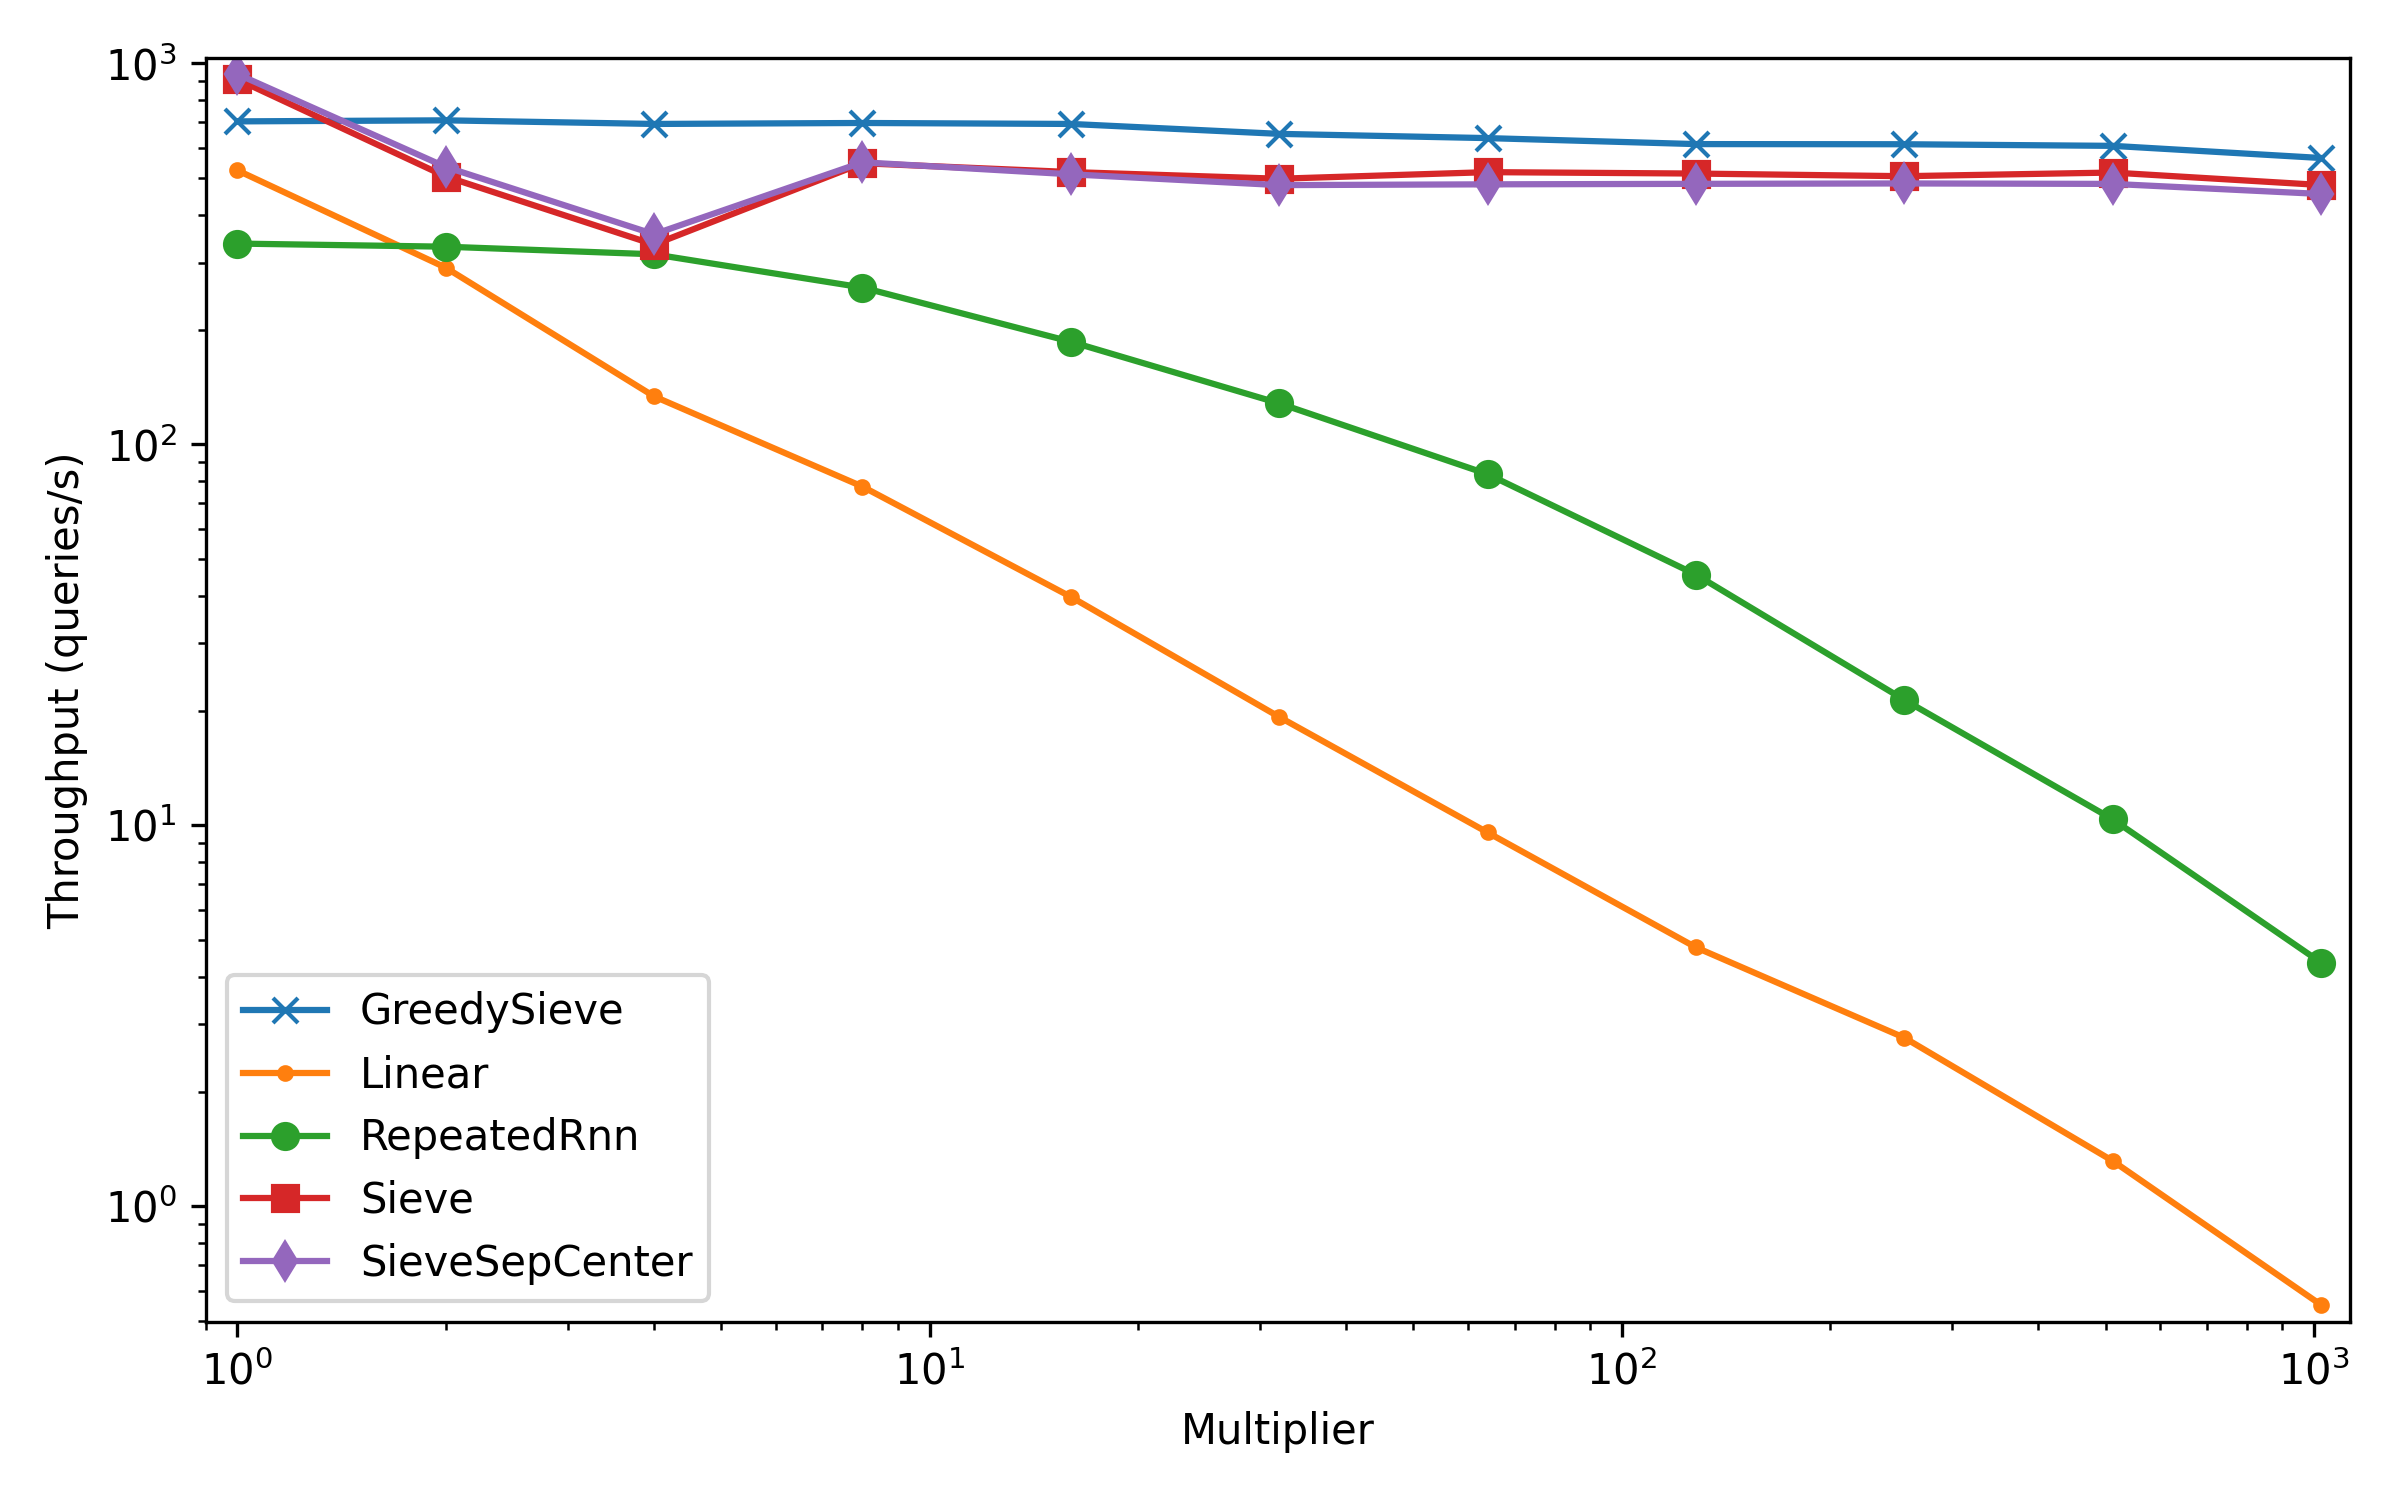
\includegraphics[width=3.4in]{images/result_plots/fashion-mnist_10_scaling.png}
    \caption{
        Fashion-mnist Scaling
    }
    \label{fig:results:fashion-mnist-scaling}
\end{figure}

% \begin{figure}[ht!]
%     \centering
%     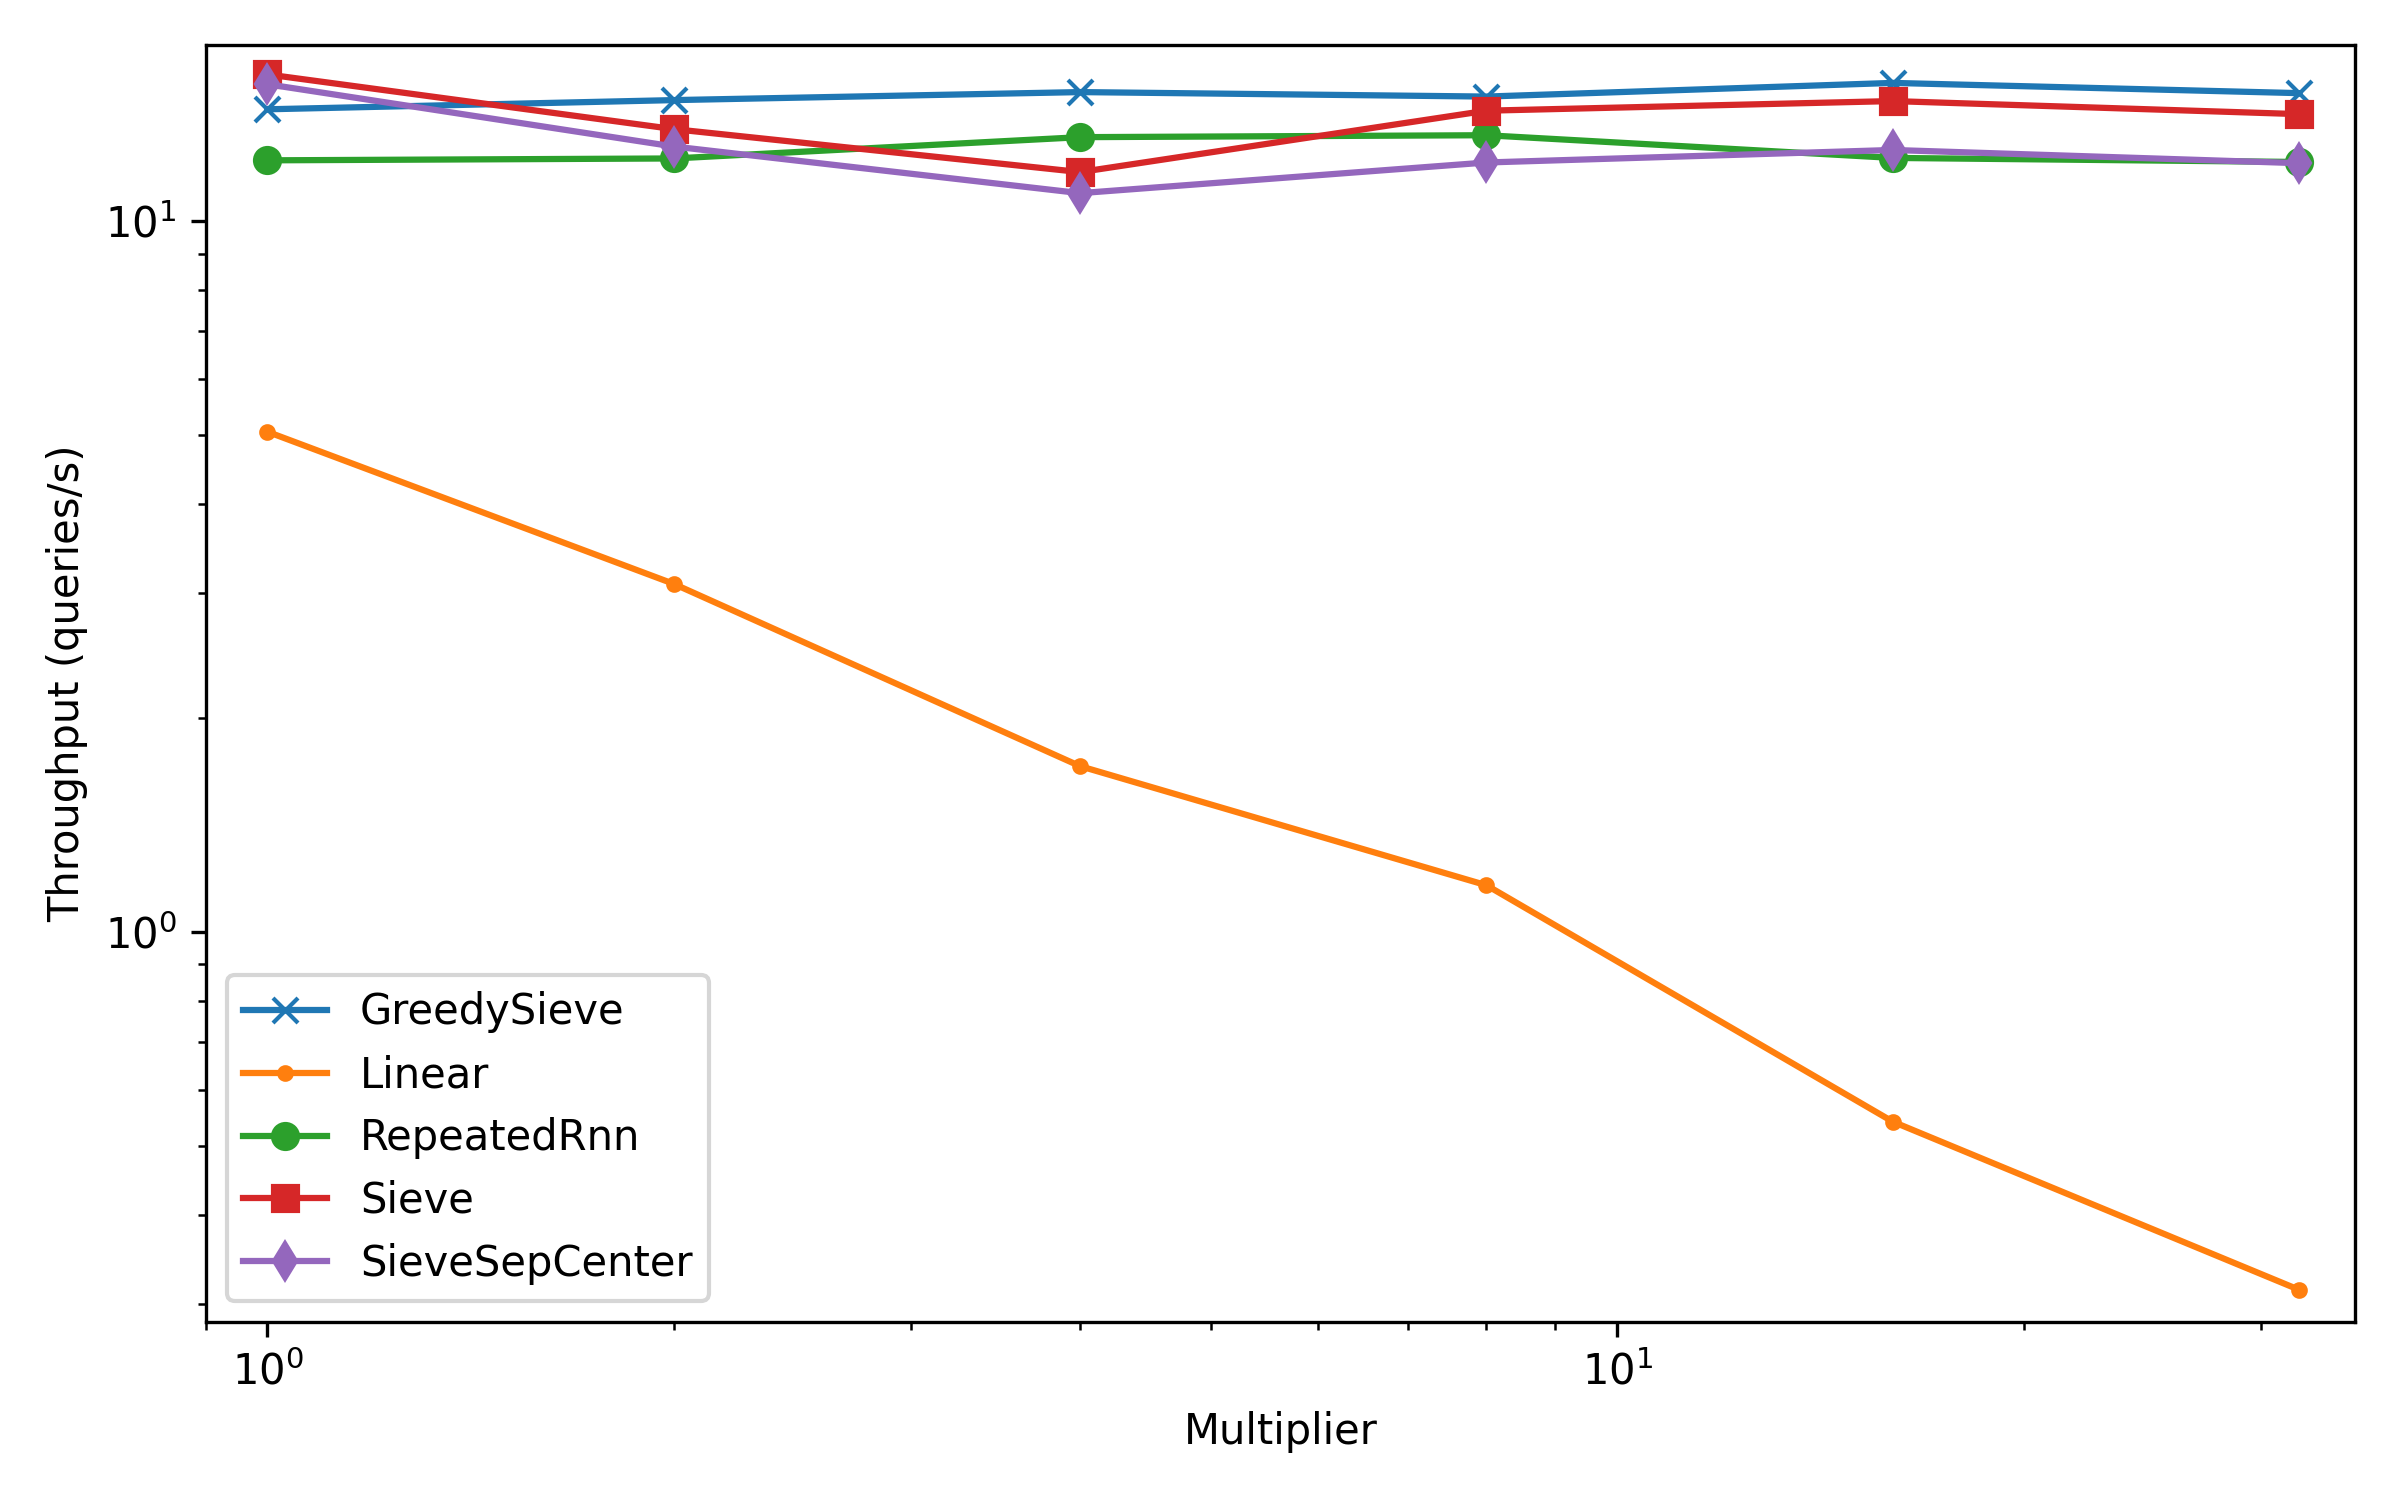
\includegraphics[width=3.4in]{images/result_plots/deep-image_10_scaling.png}
%     \caption{
%         Deep-image Scaling
%     }
%     \label{fig:results:deep-image-scaling}
% \end{figure}


\begin{figure}[ht!]
    \centering
    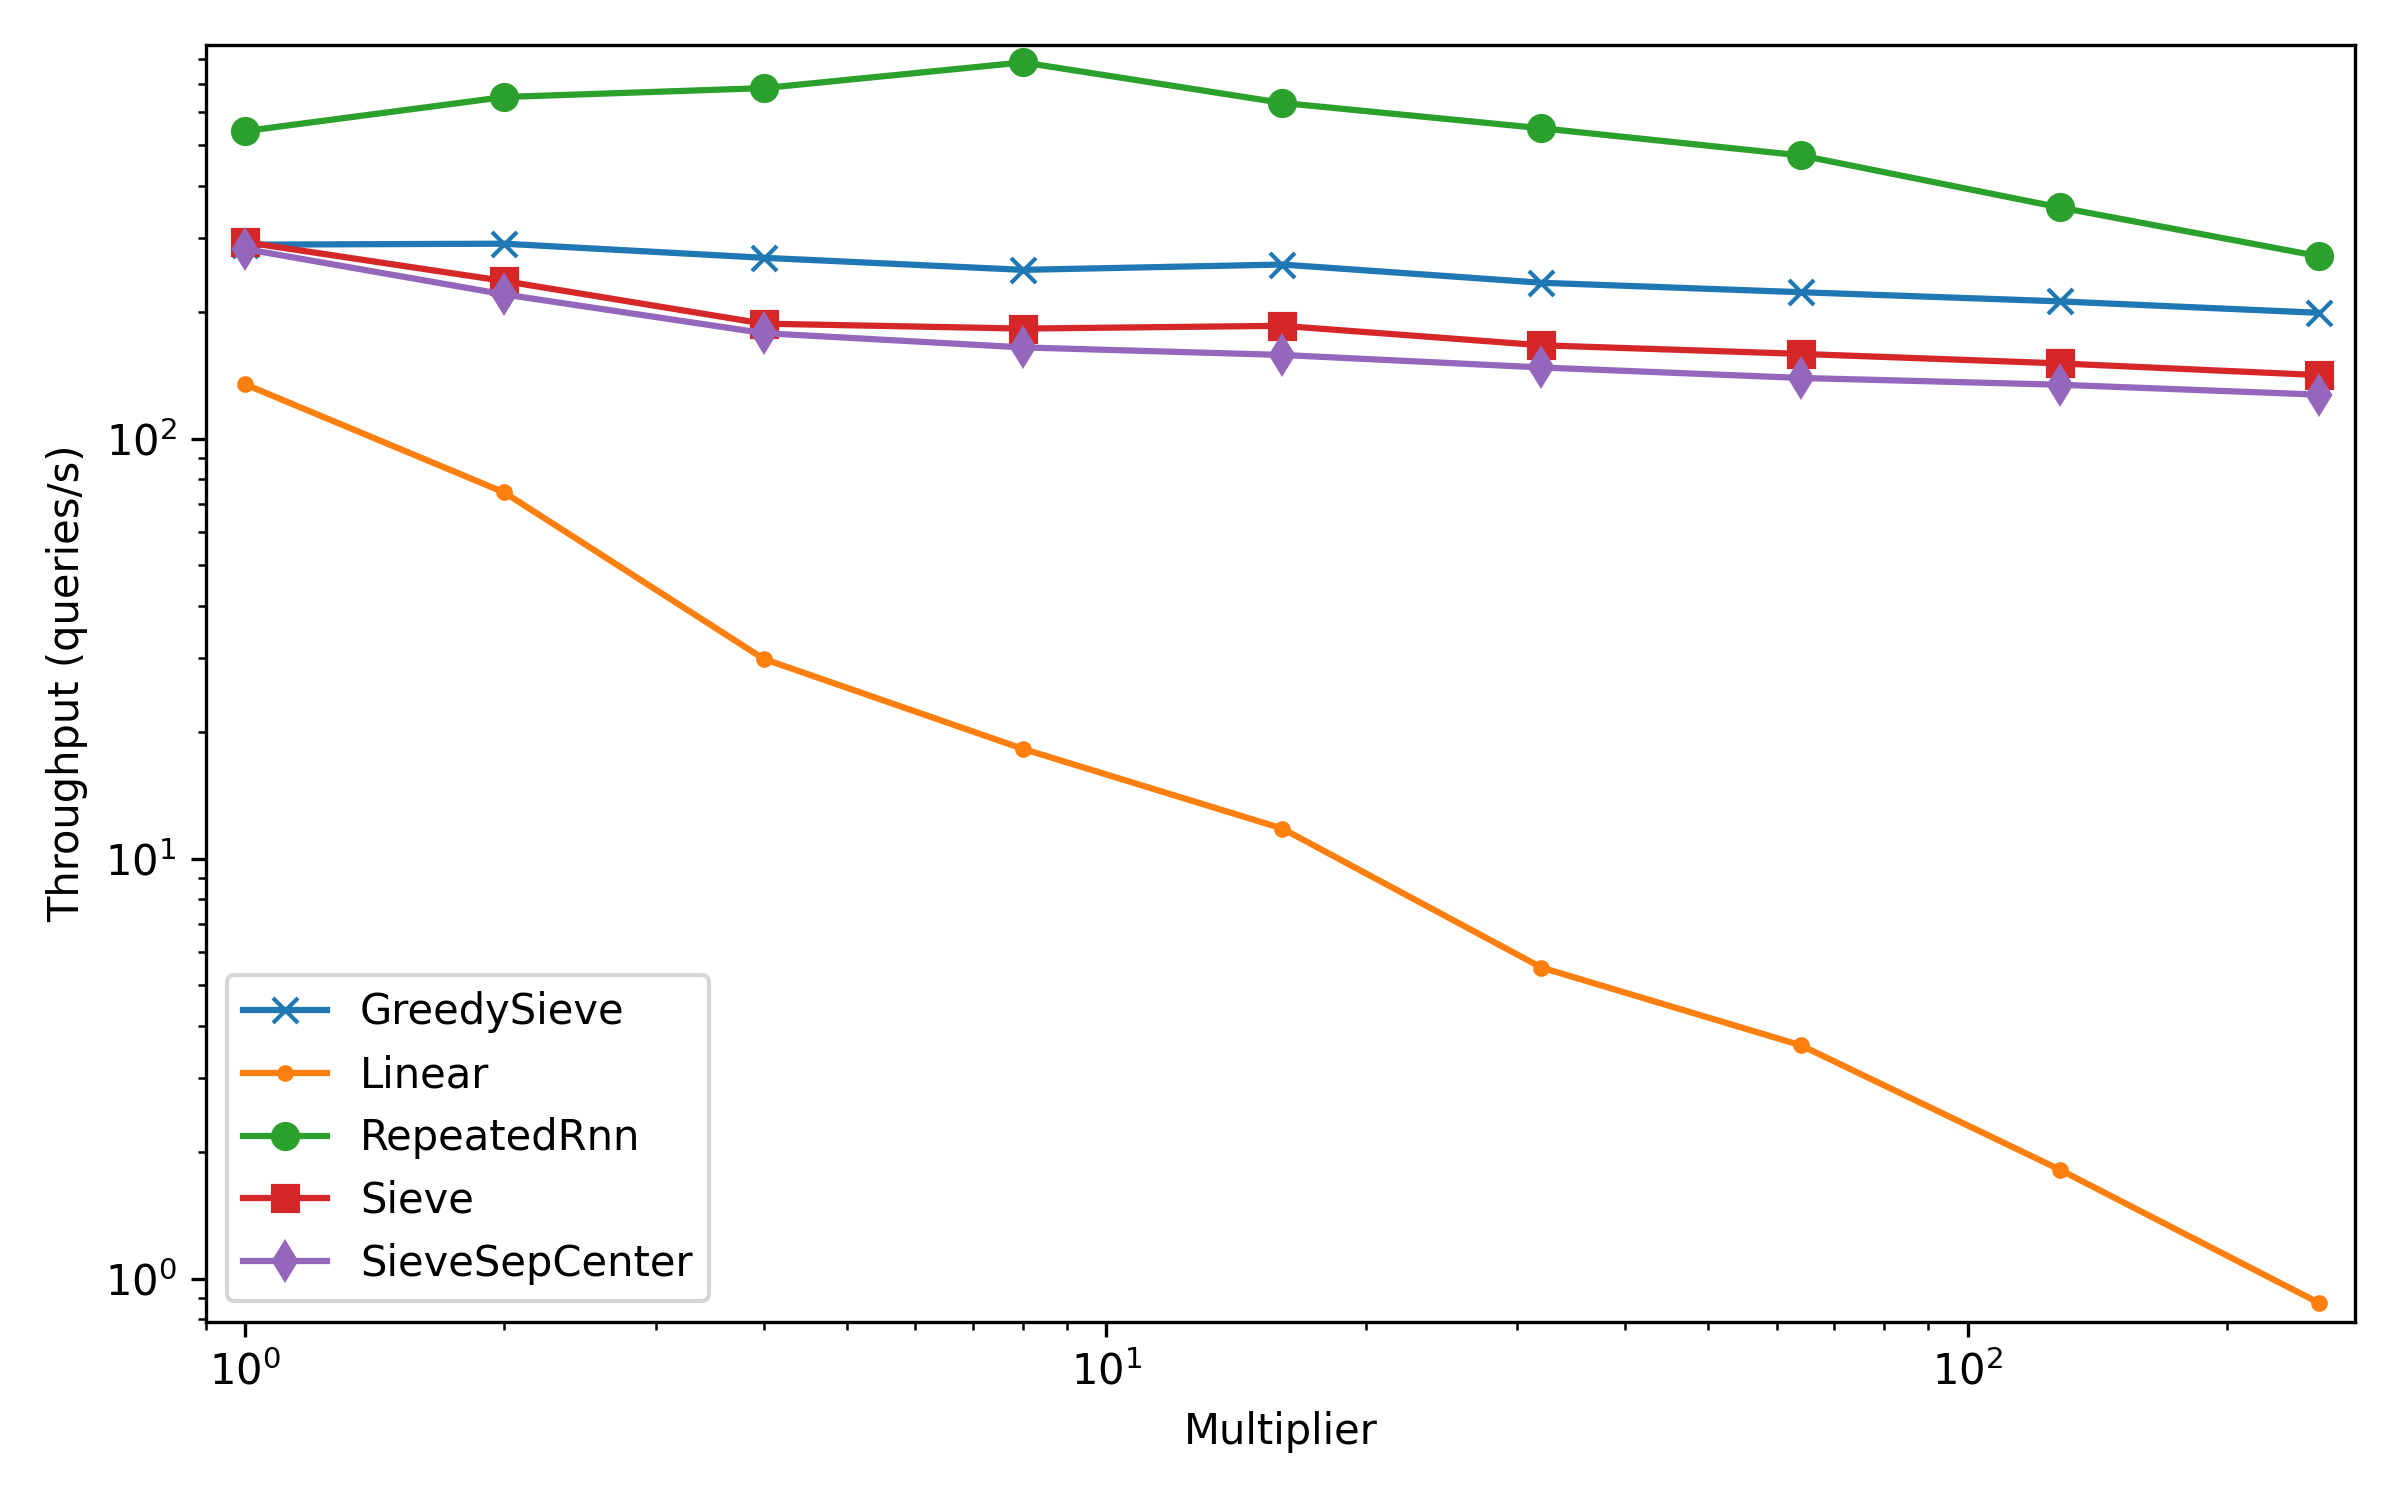
\includegraphics[width=3.4in]{images/result_plots/glove-25_10_scaling.png}
    \caption{
        Glove-25 Scaling
    }
    \label{fig:results:glove-25-scaling}
\end{figure}


\begin{figure}[ht!]
    \centering
    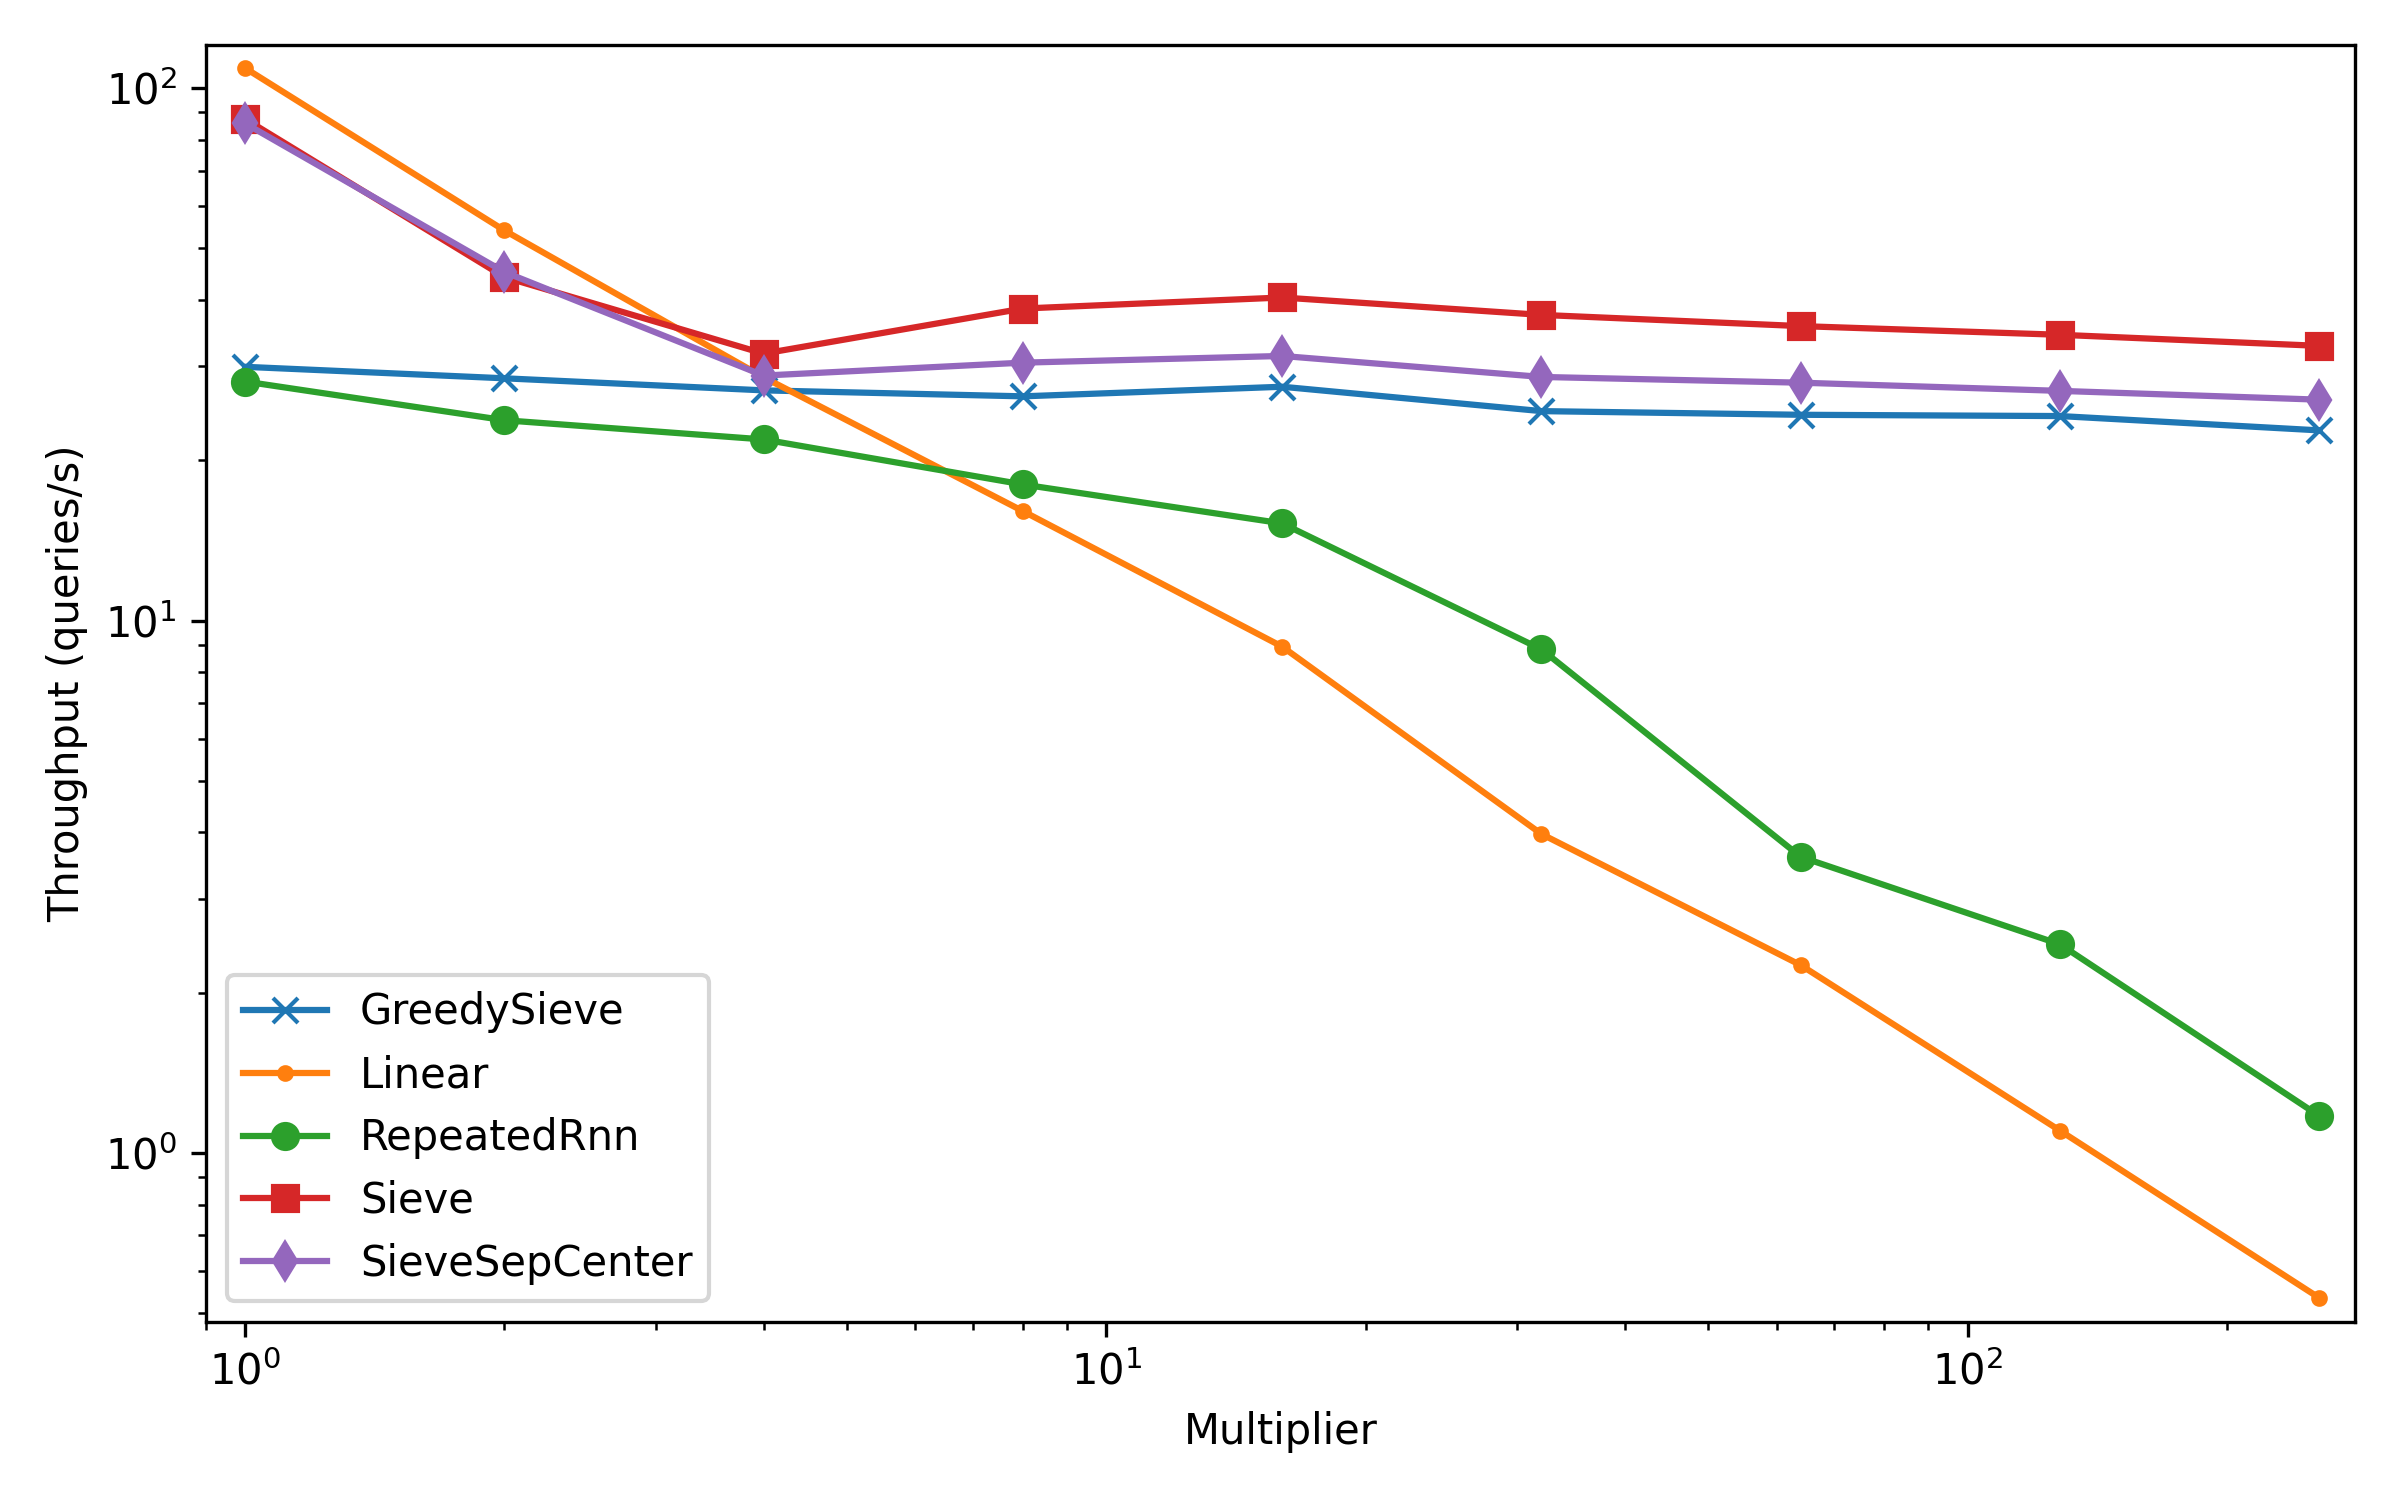
\includegraphics[width=3.4in]{images/result_plots/sift_10_scaling.png}
    \caption{
        Sift Scaling
    }
    \label{fig:results:sift-scaling}
\end{figure}

% We need to redo this plot so that we do not actually augment random datasets but instead take larger and larger 
% random datasets

\begin{figure}[ht!]
    \centering
    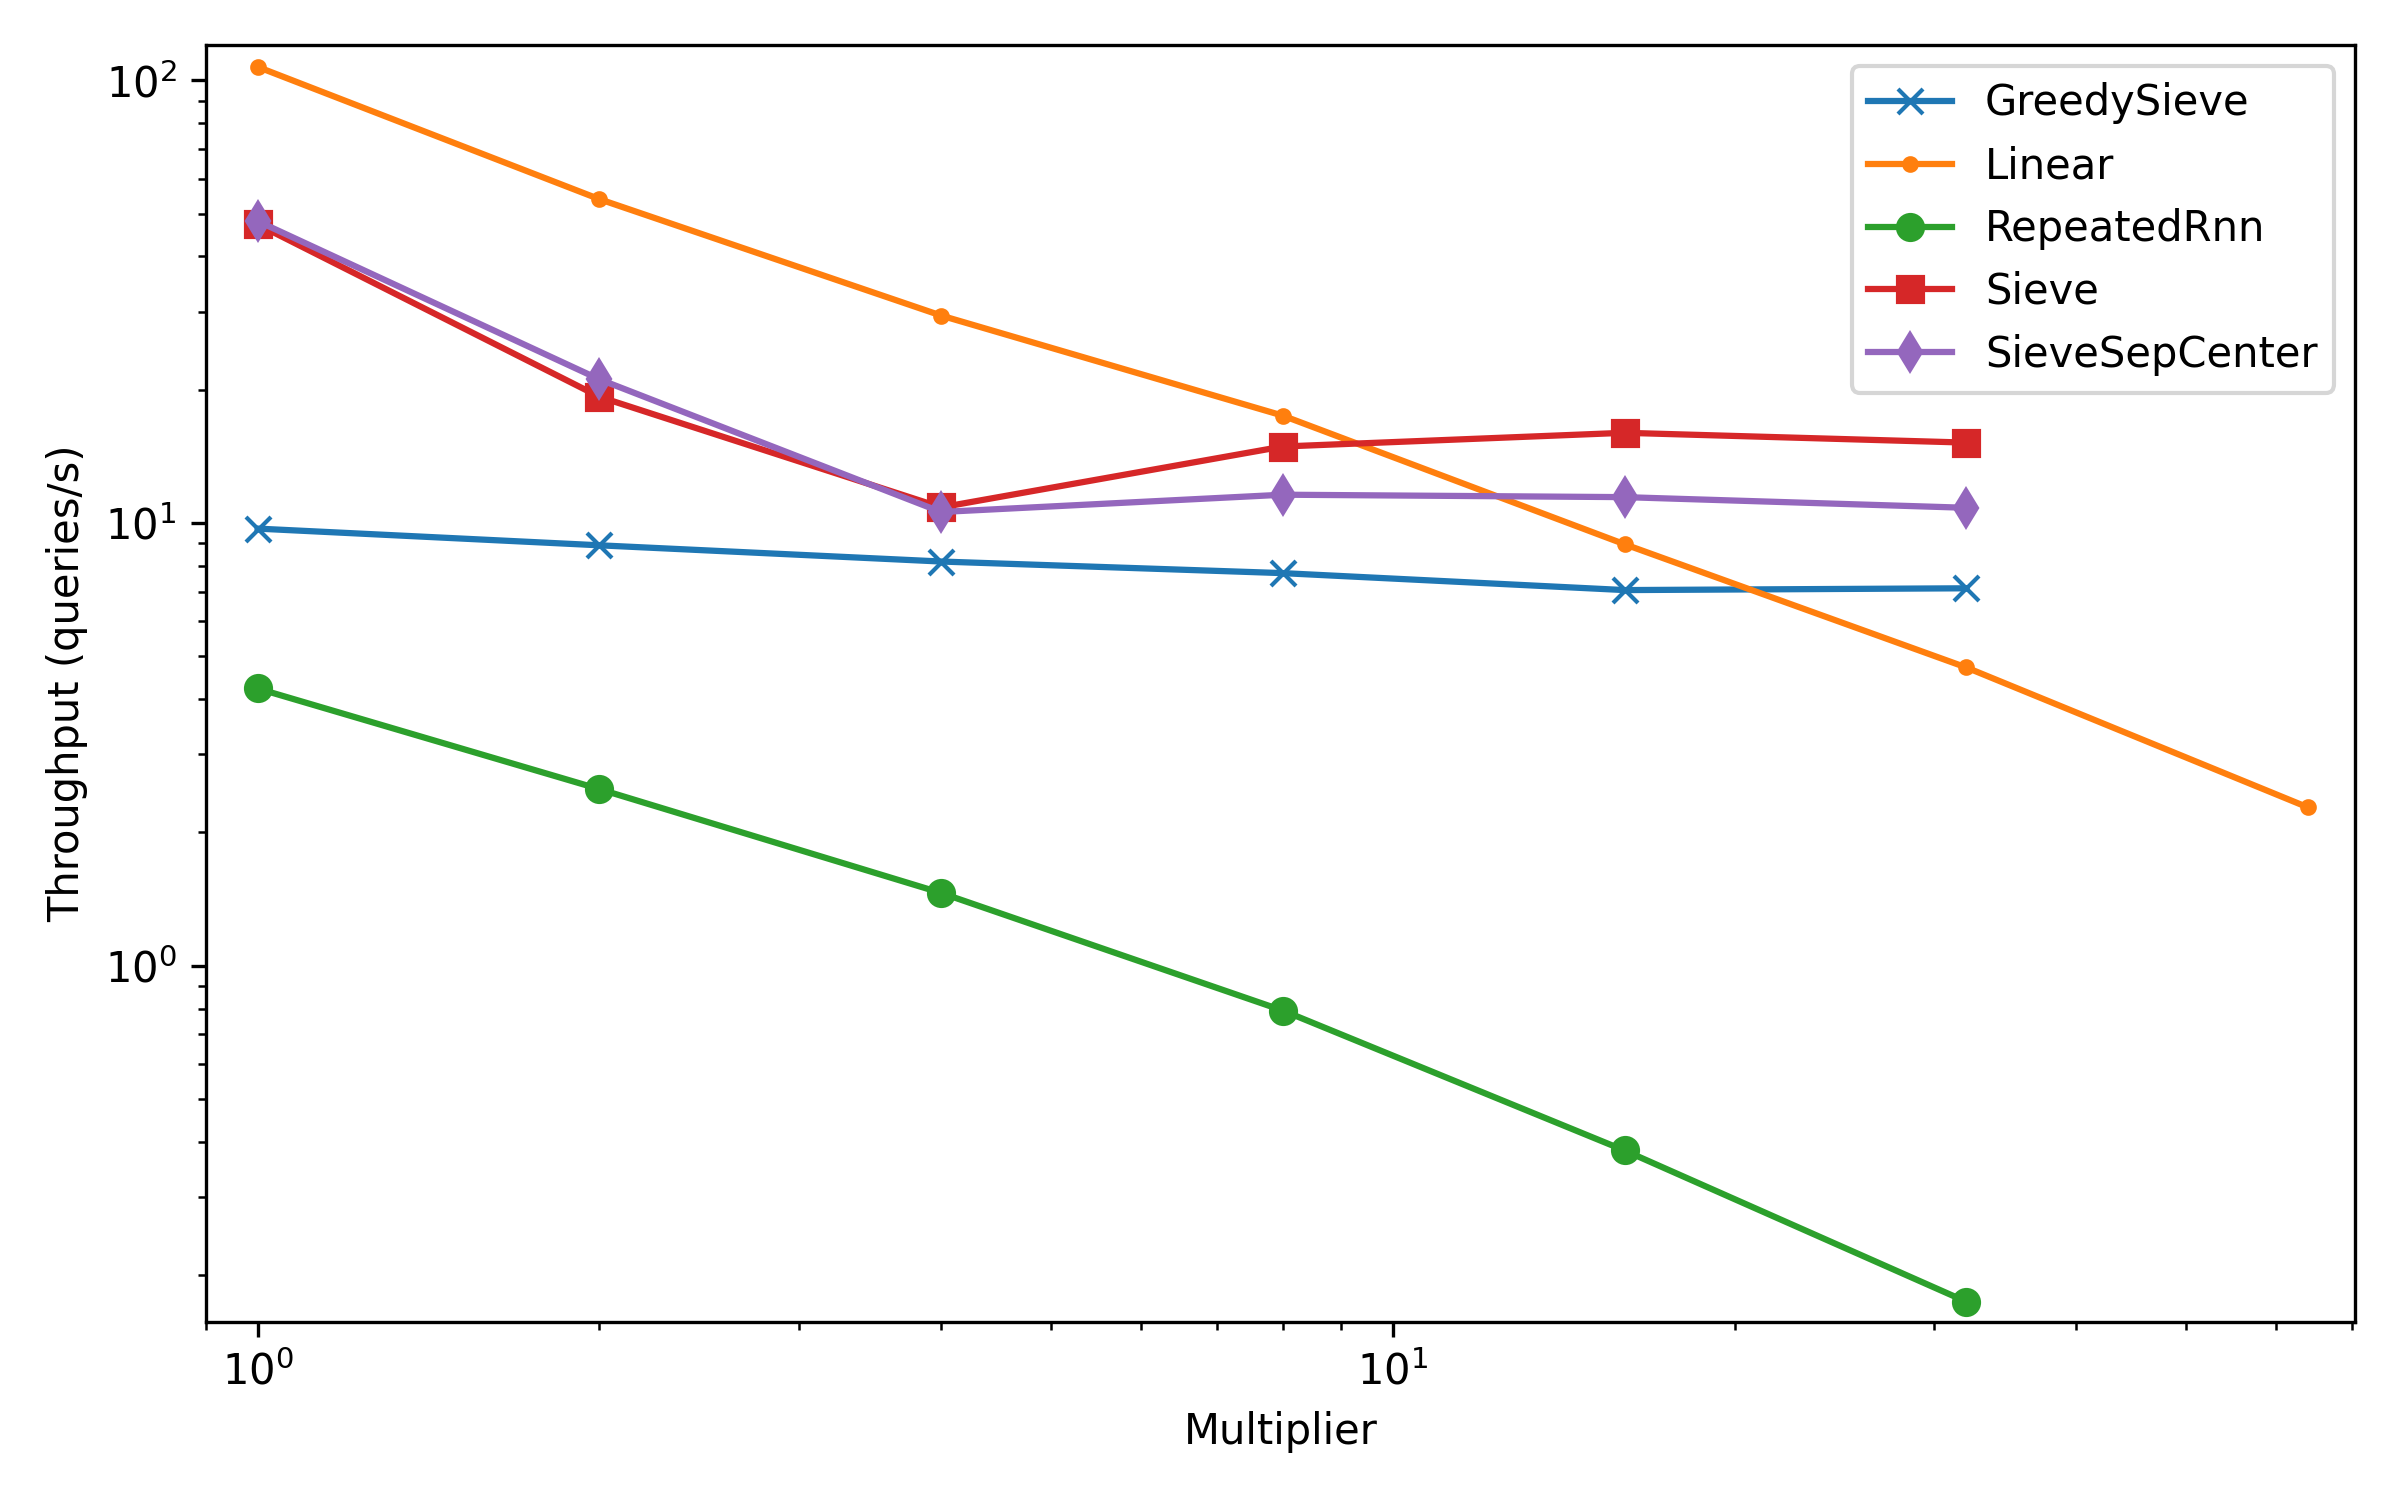
\includegraphics[width=3.4in]{images/result_plots/random_placeholder_10_scaling.png}
    \caption{
        Random Scaling
    }
    \label{fig:results:random-scaling}
\end{figure}


% We did not run any of the competitor's algorithms.
% We lifted the reported numbers from the ann-benchmarks site and their interactive plots.
% We made sure to use the same AWS instance as they did so it is a fair comparison.

% Tables \ref{table:results:ann-10} and \ref{table:results:ann-100} show the results of our benchmarks against FAISS, bruteforce-blas, and HNSW.
% The throughput values for these algorithms comes from the ANN benchmarks website's interactive plots, from which we can assess the throughput of each algorithm at a given recall value.

% We report the highest throughput value for each algorithm at a recall value of 1.0.
% We report the mean and median speedup factor of CAKES over each algorithm.
% For $k= 10$, we report a mean $7,654 \times$ (median $1,200 \times$) speedup over faiss-ivf, a mean $11,325 \times$ (median $2,821 \times$) speedup over bruteforce-blas, and a mean $485 \times$ (median $417 \times$) speedup over HNSW. 
% For $k=100$, we report a mean $4,479 \times$ (median $3,456 \times$) speedup over faiss-ivf, a mean $16,010 \times$ (median $13,548 \times$) speedup over bruteforce-blas, and a mean $403 \times$ (median $372 \times$) speedup over HNSW.

% For all datasets benchmarked in this manuscript, the auto-tuning method selected repeated $\rho$-nearest neighbor (Section~\ref{subsubsec:methods:knn-search:repeated-rnn}).

% We note that the mean and median speedup factors differ significantly for all methods, which suggests that the speedup factor is heavily dataset-dependent;
% in particular, across all algorithms, and both values of $k$, CAKES exhibits particularly high speedup factors with SIFT and GIST, under Euclidean distance.
% As GIST was designed to be a difficult dataset for classifiers~\cite{Lee2019PracticalLP}, CAKES's strong performance with this dataset is particularly encouraging.
% Further investigation of CAKES's performance on other challenging or adversarial datasets is warranted. 

% \begin{table*}[!t]
%     % \renewcommand{\arraystretch}{1.15}
%     \caption{Runtime performance (queries per second) of CAKES vs. other methods, $k=10$}
%     \label{table:results:ann-10}
%     \vskip 0.15in
%     \begin{center}
%         \begin{small}
%             \begin{sc}
%                 \begin{tabular}{|l|p{1cm}|p{1cm}|p{1cm}|p{1cm}|p{1cm}|p{1cm}|p{1cm}|p{1cm}|}
%                     \hline
%                     \textbf{Dataset}  & \multicolumn{2}{|c|}{\textbf{faiss-ivf}} & \multicolumn{2}{|c|}{\textbf{bruteforce-blas}} & \multicolumn{2}{|c|}{\textbf{hnsw(faiss)}} & \multicolumn{2}{|c|}{\textbf{CAKES}} \\
%                     \cline{2-9}
%                     &               Recall & QPS      & Recall & QPS    & Recall & QPS    & Recall & QPS \\
%                     \hline
%                     fashion-mnist & 1.000  & 188.03    & 1.000 & 52.91  & 1.000* & 339.74 & 1.000 & 141,800 \\
%                     \hline
%                     gist          & 1.000 & 3.55  & 1.000 & 2.63        & 0.953 & 149.58  & 1.000 & 76,420 \\
%                     \hline
%                     glove-25      & 1.000 & 78.78  & 1.000 & 33.52      & 1.000 & 552.67  & 0.798 & 94,580 \\
%                     \hline
%                     glove-100     & 1.000 & 21.16  & 1.000 & 16.52      & 0.998 & 155.90  & 0.904 & 4,566 \\
%                     \hline
%                     sift          & 1.000 &  24.52 & 1.000 & 16.40      & 1.000 & 275.07  & 1.000 & 357,400 \\
%                     \hline
%                 \end{tabular}
%             \end{sc}
%         \end{small}
%     \end{center}
%     \vskip -0.1in
% \end{table*}

% \begin{table*}[!t]
%     % \renewcommand{\arraystretch}{1.15}
%     \caption{Runtime performance (queries per second) of CAKES vs. other methods, $k=100$. Other methods did not report results for glove-25. Asterisk on recall value indicates that the algorithm had imperfect recall greater than or equal to 0.9995.}
%     \label{table:results:ann-100}
%     \vskip 0.15in
%     \begin{center}
%         \begin{small}
%             \begin{sc}
%                 \begin{tabular}{|l|p{1cm}|p{1cm}|p{1cm}|p{1cm}|p{1cm}|p{1cm}|p{1cm}|p{1cm}|}
%                     \hline
%                     \textbf{Dataset}  & \multicolumn{2}{|c|}{\textbf{faiss-ivf}} & \multicolumn{2}{|c|}{\textbf{bruteforce-blas}} & \multicolumn{2}{|c|}{\textbf{hnsw(faiss)}} & \multicolumn{2}{|c|}{\textbf{CAKES}} \\
%                     &                    Recall & QPS  & Recall & QPS     & Recall & QPS      & Recall & QPS \\
%                     \hline
%                     fashion-mnist  & 1.000 & 111.47    & 1.000* & 16.02   & 1.000* & 277.80   & 1.000 & 71,370 \\ 
%                     \hline
%                     gist           & 1.000 & 2.70      & 1.000* & 0.80    & 0.995 & 59.71     & 1.000 & 29,090 \\
%                     \hline
%                     glove-25       & -- & --           & --     & --      & -- & --           & 0.851 & 49,350 \\
%                     \hline
%                     glove-100      & 1.000* &  19.04   & 1.000* & 7.52    & 0.987 & 92.58     & 0.905 & 4,384 \\
%                     \hline
%                     sift           & 1.000 &  23.50    & 1.000  & 6.51    & 1.000* & 179.14   & 1.000 & 147,400 \\                                                 
%                     \hline
%                 \end{tabular}
%             \end{sc}
%         \end{small}
%     \end{center}
%     \vskip -0.1in
% \end{table*}


% \begin{table*}[!t]
%     % \renewcommand{\arraystretch}{1.15}
%     \caption{Runtime performance (queries per second) of CAKES and Speedup Factor over Naive Linear Search, $k=10$}
%     \label{table:results:ann-alt-10}
%     \vskip 0.15in
%     \begin{center}
%         \begin{small}
%             \begin{sc}
%                 \begin{tabular}{|l|l|l|l|l|}
%                     \hline
%                     \textbf{Dataset} & \textbf{CAKES Throughput} & \textbf{Speedup Factor over Linear} \\
%                     \hline
%                     deep-image       & 232.1                     & 37.2      \\
%                     \hline
%                     mnist            & 129,300                   & 101.9      \\
%                     \hline
%                     glove-50         & 10,950                    & 12.28      \\
%                     \hline 
%                     glove-200        & 2,290                     & 8.55     \\
%                     \hline
%                     lastfm           & 13,950                    & 4.55           \\
%                     \hline
%                 \end{tabular}
%             \end{sc}
%         \end{small}
%     \end{center}
%     \vskip -0.1in
% \end{table*}


% \begin{table*}[!t]
%     % \renewcommand{\arraystretch}{1.15}
%     \caption{Runtime performance (queries per second) of CAKES and Speedup Factor over Naive Linear Search, $k=100$}
%     \label{table:results:ann-alt-100}
%     \vskip 0.15in
%     \begin{center}
%         \begin{small}
%             \begin{sc}
%                 \begin{tabular}{|l|l|l|l|l|l|}
%                     \hline
%                     \textbf{Dataset} & \textbf{CAKES Throughput} & \textbf{Speedup Factor over Linear} \\
%                     \hline
%                     deep-image        & 157.3                    & 25.74                               \\                            
%                     \hline
%                     mnist             & 71,090                   & 56.63                               \\
%                     \hline
%                     glove-50          & 8,867                    & 9.84                                \\
%                     \hline 
%                     glove-200         & 2,264                    & 8.49                                \\
%                     \hline
%                     lastfm            & 13,950                   & 4.55                                \\
%                     \hline
%                 \end{tabular}
%             \end{sc}
%         \end{small}
%     \end{center}
%     \vskip -0.1in
% \end{table*}

    \section{Discussion and Future Work}
\label{sec:discussion-and-future-work}

We have presented CAKES, a set of three algorithms for fast $k$-NN search that are generic over a variety of distance functions.
CAKES's algorithms are exact when the distance function in use is a metric (see definition in Section~\ref{sec:methods}).
Even under cosine distance, which is not a metric, CAKES's algorithms exhibit nearly perfect recall.
CAKES's algorithms are designed to be most effective when the data uphold the manifold hypothesis, or in other words, when the data are constrained to a low-dimensional manifold even when embedded in a high-dimensional space.
As a consequence, these algorithms do not perform well on data with random distributions, because of the absence of a manifold structure.
In Figure~\ref{fig:results:lfd-plots}, we show the extent to which each dataset we tested exhibits a manifold structure, as quantified by the percentiles of LFD.
As expected, our results from Figure~\ref{fig:results:scaling-plots} indicate that CAKES's algorithms scale sub-linearly with cardinality on datasets with low LFD, and scale linearly on datasets with high LFD.

CAKES's performance on Sift against that on the Random dataset illustrates this phenomenon well. As seen in Figures~\ref{fig:results:random-lfd}~and~\ref{fig:results:sift-lfd}, the LFD of the Random dataset is much higher than that of Sift, even though both datasets have the same cardinality and dimensionality.
This is unsurprising, given that the Random dataset is uniformly distributed, while Sift is not.
On the Random dataset, CAKES's speed decreases linearly as the multiplier increases, while with Sift, Depth-First Sieve and Breadth-First Sieve both exhibit nearly constant throughput.
While Repeated $\rho$-NN does not exhibit near-constant throughput with Sift, throughput decreases much more slowly than it does with the Random dataset.
Since these two datasets have the same cardinality and embedding dimension, the aforementioned discrepancies highlight how manifold structure affects algorithm performance.


We emphasize that although CAKES's algorithms are slower on the Random dataset, their recalls remain perfect.
Figure~\ref{fig:results:scaling-plots} also shows that HNSW and ANNOY have near-constant throughput as the multiplier increases, but their recall continues to decrease as the multiplier increases.
This, coupled with the increasing time and space cost of building the indices for HNSW and ANNOY, makes these algorithms unsuitable for real-world applications in which the datasets are growing exponentially.
CAKES's tree is orders of magnitude faster and less memory-intensive to build, and CAKES's algorithms, while slower than HNSW and ANNOY, still show near-constant scaling as well as perfect recall.

When written with the same notation as used in Section~\ref{sec:methods:knn-search:complexity-of-sieve-methods}, we see that the time complexity of Repeated $\rho$-NN is $\mathcal{O}(\tfrac{T}{\lceil d \rceil} + L)$, where $T$ is the time complexity of tree-search and $L$ is the time complexity of leaf-search.
Even though Repeated $\rho$-NN has the least time cost (compare to $\mathcal{O}(T\log{(T+L)} + L\log{(T+L)})$ for Breadth-First Sieve and $\mathcal{O}(T\log{T} + L\log{k})$ for Depth-First Sieve) of the three CAKES algorithms, it is not always the fastest algorithm empirically.
We believe that some of this discrepancy can be explained by the fact that if Repeated $\rho$-NN significantly ``overshoots'' the correct radius for $k$ hits ($\rho_k$) during tree-search, leaf-search will require looking at more points, rendering the true scaling factor higher than that in Equation~\ref{eq:methods:repeated-rnn-complexity}.
This overshot can occur when the LFDs of clusters near the query are not concentrated around their expectation.
For example, if most clusters near the query have very low LFD except for one anomaly with very high LFD,
the harmonic mean LFD $\mu$ can still be low, so the factor of radial increase in (Equation)~\ref{eq:methods:repeated-rnn-factor} may be much larger than necessary for guaranteeing $k$ hits.
This suggests that rather than using the reciprocal of the harmonic mean LFD in~\ref{eq:methods:repeated-rnn-factor}, we may achieve better results with a mean that is more sensitive to high outliers, such as the geometric mean.
We leave it as an avenue for future work to characterize when Repeated $\rho$-NN significantly overestimates the correct radius $\rho_k$ and to improve upon the factor of radial increase in Equation~\ref{eq:methods:repeated-rnn-factor} so that this occurs less frequently and with less severity.

As the previous paragraph suggests, the fastest CAKES algorithm varies by dataset.
For example, on Glove-25, Repeated $\rho$-NN exhibits the highest throughput of any CAKES algorithm, despite having the lowest throughput of the three on Sift and Fashion-Mnist.
On Silva, Repeated $\rho$-NN is comparable to the other CAKES algorithms at low multipliers, but becomes the fastest at the higher multipliers.
When we view these results in light of the LFD plots in Figure~\ref{fig:results:lfd-plots}, we realize that Repeated $\rho$-NN appears to be the fastest CAKES algorithm on datasets where a large proportion of the data have a very low LFD, such as Glove-25 and Silva.
This trend is unsurprising, given that Repeated $\rho$-NN relies on a low LFD around the query in order to quickly estimate the correct radius for $k$ hits.
These findings suggest that Repeated $\rho$-NN is the most ``sensitive'' to the manifold structure of the dataset.
Exploring this sensitivity is a potential avenue for future study, as it remains to learn at what LFD Repeated $\rho$-NN transitions away from being the fastest CAKES algorithm, and whether this transition is sharp.

While the fastest CAKES algorithm varies by dataset, we note that on all three ANN-benchmark datasets (Fashion-Mnist, Glove-25, and Sift), Depth-First Sieve and Breadth-First Sieve show nearly constant throughput as the cardinality increases.
This observation warrants further investigation, but it is especially promising given that both algorithms consistently outperform linear search for high cardinalities.
Finally, we emphasize that the variation in performance of our algorithms across different datasets and cardinalities supports our use of an auto-tuning function (as discussed in Section~\ref{sec:methods:auto-tuning}) to select the best algorithm for a given dataset.
Future work is needed to better characterize those datasets for which each algorithm performs best, but our results suggest that a more sophisticated auto-tuning function could be developed to select the fastest algorithm based on the properties of the dataset.

We also stress that CAKES's algorithms are designed to work well for \textit{big} data, and our results support this claim;
we observe that while linear search can outperform CAKES on datasets with small cardinality, CAKES always overtakes linear search at a large enough cardinality for each of the ANN-benchmark datasets we tested.
Moreover, we observe that CAKES's algorithms outperform linear search at a lower cardinality when the dataset has a lower LFD.
For example, Sift has much higher LFD than Fashion-Mnist and Glove-25, and we observe that CAKES overtakes linear search at a cardinality of $10^7$ for Sift, as opposed to about $10^5$ and $10^6$ for Fashion-Mnist and Glove-25, respectively.
For the Random dataset, which has the highest LFD, CAKES's algorithms \textit{never} outperform linear search.
These observations support our claim that CAKES performs well on datasets that arise from constrained generating phenomena, even as the cardinalities of these datasets grow exponentially. 




The questions raised by this study suggest several additional avenues for future work.
A comparison across more datasets is in order, as is further analysis with other distance functions that existing methods, such as FAISS, HNSW and ANNOY, do not support. These include Wasserstein distance~\cite{vallender1974calculation} for probability distributions (particularly for high dimensional distributions) and Tanimoto distance~\cite{bajusz2015tanimoto} for comparing molecular structures by their maximal common subgraphs.
Incorporating these or other distance functions in CAKES requires only that a Rust implementation of the distance function be provided.

Additionally, we intend to improve the data augmentation process described in Section~\ref{sec:methods:synthetic-data} to better preserve the topological structure of the underlying dataset. 
In particular, we expect that favoring augmentation along the first principal components of the local manifold may allow for more realistic data augmentation. 

We also plan to investigate hierarchical data compression by representing differences at each level of the binary tree, particularly for string or genomic data, where all differences are discrete.
Such an encoding would allow us to store the data in a compressed format, and to perform search on the compressed data without decompressing it.
This would allow us to perform fast search on datasets that are too large to fit in memory.
An exploration of compression and compressed search is another avenue for future work.

We also would like to explore the use of CAKES in a streaming environment.
This would require the ability to perform ``online'' updates to the tree as points are added to or deleted from the dataset.
Such online updates would take advantage of the fast search algorithms provided by CAKES.  % and would allow us to have our cake and eat it, too.
CAKES can also be used to extend anomaly detection in CHAODA~\cite{ishaq2021clustered}.
We could add to CHAODA's ensemble of graph-based anomaly detection methods by using the distribution of distances among the $k$ nearest neighbors of cluster centers.

CLAM and CAKES are implemented in Rust and the source code is available under an MIT license at https://github.com/URI-ABD/clam.


    \section*{Acknowledgments}
    The authors thank the members of the University of Rhode Island's Algorithms for Big Data research group for their helpful comments throughout the development of this work.

    % \afterpage{\clearpage}
    \FloatBarrier
    \bibliographystyle{ACM-Reference-Format}
    \bibliography{references}
\end{document}
